\documentclass[]{beamer}
\resetcounteronoverlays{saveenumi}
\usepackage{beamerthemesplit}  
\usepackage{outlines}
\usepackage{comment}
\usepackage{lscape}
\usepackage{tikz}
\usetikzlibrary{spy}
\usepackage{pgfplots} 
\usepackage{amsmath} 

\usepackage{subcaption}
\usepackage{movie15}
\usepackage{graphicx}
\usepackage{overpic,picture}
\usepackage{hyperref}
\usepackage{pdfpages}
\usepackage{graphicx}% http://ctan.org/pkg/graphicx
\usepackage{booktabs}% http://ctan.org/pkg/booktabs
\usepackage[T1]{fontenc}
\usepackage[utf8]{inputenc}
\usepackage{multirow}                    
\usepackage{ragged2e}
\usepackage{etoolbox}
\usepackage{lipsum}
\usepackage{tabularx}  
\usepackage{outlines}
\usecolortheme{beaver}
\usetheme{Warsaw}
\setbeamertemplate{page number in head/foot}[totalframenumber]

\usepackage{lmodern}
\usepackage[beamer,customcolors]{hf-tikz}

\tikzset{hl/.style={
    set fill color=red!80!black!40,
    set border color=red!80!black,
  },
}



\apptocmd{\frame}{}{\justifying}{}

\newcolumntype{C}{>{\Centering\arraybackslash}X}


\title[The Case of Divided Cities in Europe]{\small Bring Together What Belongs Together: 
\\The Case of Divided Cities in Europe}
%\subtitle{An Introduction}
\author[]{\small Ketevani Kapanadze^{\dagger}}
\vspace{2cm}

\institute[]{\small ^{\dagger}$European Research University (ERUNI)$
\\ \vspace{1cm}
Conference of the Czech Economic Society
} 

\date{}

\begin{comment} 
\title[]{\small Bring Together What Belongs Together:
\\The Case of Divided Cities in Europe}   

\author[ ]
{
\small Ketevani Kapanadze^{\dagger} 
\newline {}
\vspace{1.5cm}} 

\institute{\small \textit{Border, Politics and Policies: Using Data to Power Border Research
\\Jean Monnet Network Conference}
\vspace{1cm}
\\ ^{\dagger}$Charles University, Faculty of Law$
{
\newline {}  } }   
\date{{
\newline {}  } }
\setbeamercovered{highly dynamic}
\end{comment}



\newcounter{saveenumi}
\newcommand{\seti}{\setcounter{saveenumi}{\value{enumi}}}
\newcommand{\conti}{\setcounter{enumi}{\value{saveenumi}}}
\begin{document}
\beamertemplatenavigationsymbolsempty

\begin{frame}
  \titlepage 
\end{frame}


\begin{frame}{Outline}
\begin{itemize}
    \item Literature \& Motivation
    \item History of Divided Cities in Europe
    \item Data 
    \item Empirical Results 
    \item Channels 
    \item Take-aways
\end{itemize}
    
\end{frame}


\begin{frame}{Literature \& Motivation}
What are the main drivers for the spatial distribution of economic activities \textbf{within} cities? 

\vspace{0.5cm}
Why do economies cluster? 
\begin{itemize}
    \item First degree geography - natural advantages or natural resources  
    \item Second degree geography - lower transportation cost

\newline
\vspace{0.5cm}
\begin{itemize}
    \item  US cities - \textit{Baum-Snow et al. (2005), Arzaghi \&  Henderson (2008), Rossi-Hansberg et al. (2010) and  Brooks \&  Lutz (2019) }
    \item London - \textit{Heblich et al. (2020)}
    \item Berlin - \textit{Ahlfeldt et al. (2015)}
\vspace{0.5cm}
    
\end{itemize}
 \end{itemize}
\end{frame}

\begin{frame}{My paper : The Case of Divided European Cities}
A quasi-natural experiment on the opening of borders (under Schengen) within European divided border cities that were historically a single urban unit.
 \vspace{1cm}
 \\Multinational perspective:
\begin{itemize}
    \item Differences in Languages \&  Cultures
    \item Borderless Market (EU) \& Borderless People (Schengen)
\end{itemize}
\end{frame}
 




\begin{frame}{European Integration}
\small
\\\textit{{\textbf{Across}} European regions and cities:} 
\begin{itemize}
\justifying
%\item The effects of broader market access due to European integration have been studied \textit{\textbf{across}} European regions and cities, with a special focus on border areas - 
\item free movement of goods, services, and capital (EU) - \textit{Braakmann and Vogel (2011); Brakman et al. (2012); Brülhart et al. (2018)}
\item free movement of persons (SCH) - \textit{Mitze and Breidenbach (2018); Heider (2019); Kapanadze (2021)}
%\item \textit{Common Finding:} economic activities are unevenly distributed \textit{across} regions and cities in the course of European integration 
\end{itemize}
\vspace{0.5cm}
\\\Rightarrow ${Cross-city analysis raises an important question about \textbf{within} city distribution: \textit{did  European integration affect the internal structure of cities?}}$ 

% Do spatial concentrations have deep historical roots in Europe?
\begin{itemize}
\justifying
%\item  In contrast to all the previous studies on European integration, which exploit variation \textbf{\textit{across}} regions or cities, my focus and contribution are on the effect of European integration on economic activities \textit{\textbf{within}} cities
%\item My contribution: the effects of EU and Schengen enlargements  on economic activities \textit{\textbf{within divided}} cities
%\item U.S. cities - \textit{Baum-Snow et al. (2005); Arzaghi and Henderson (2008)};  Berlin - \textit{Ahlfeldt et al. (2015)}; London - \textit{Heblich et al. (2020)}
\end{itemize}
\end{frame}


\begin{frame}{{Divided city of Cieszyn (PL) \& Český Těšín (CZ)}}
    \begin{figure}
  \begin{tabular}{c|c} %vertical line I added | between cc
  \subcaptionbox{In 1910 - one (united) city}{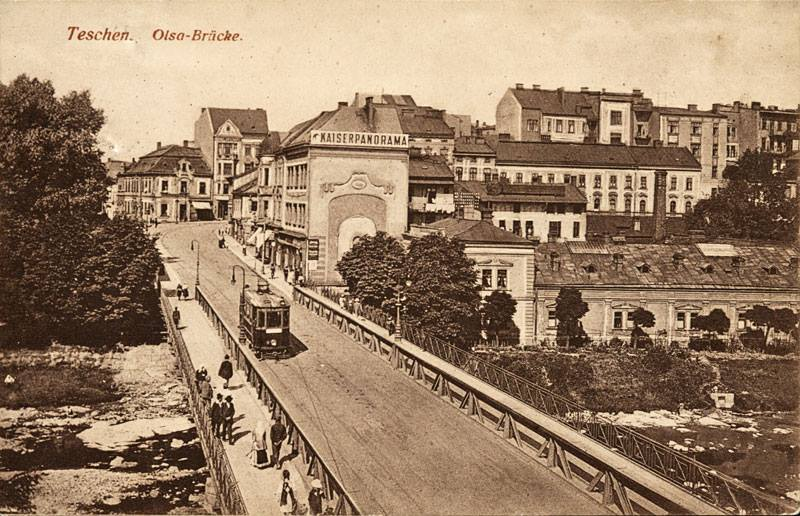
\includegraphics[scale=0.18]{1.jpg}}&
  \subcaptionbox{In 1950 - divided \& borders}{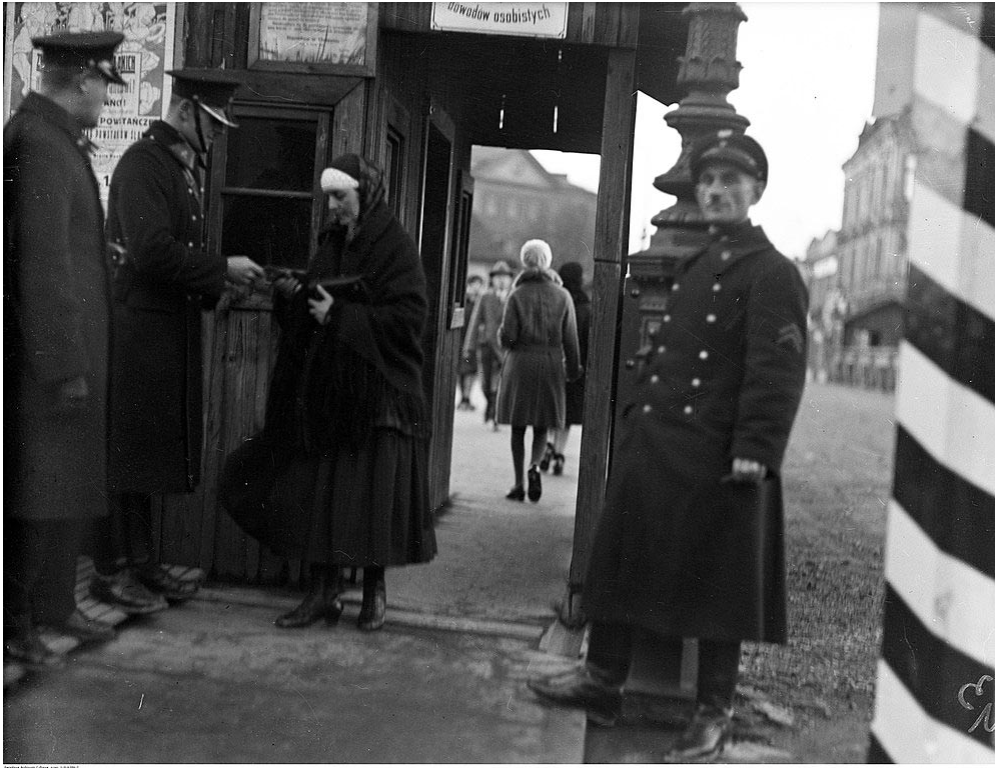
\includegraphics[scale=0.25]{Screenshot 2022-11-29 at 16.01.44.png}}\\
  \hline
  \subcaptionbox{In 2005 - still border controls}{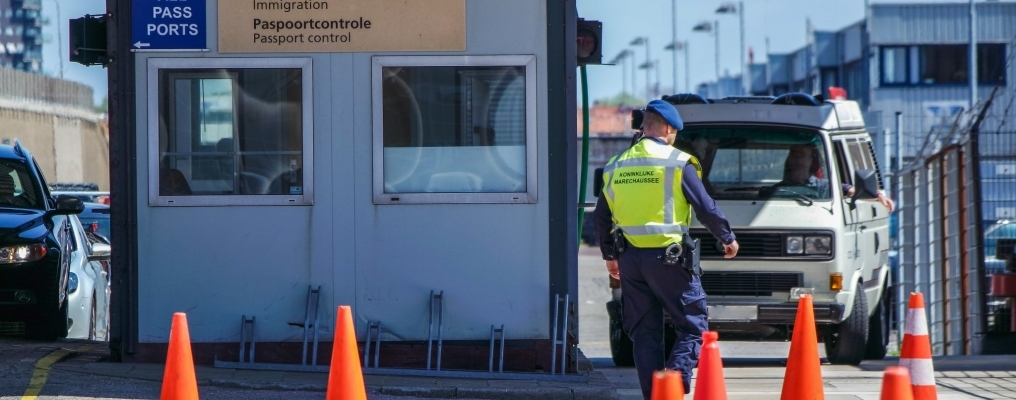
\includegraphics[scale=0.2]{AdobeStock_83908494-scaled-pkk4j6s2slao3i14bvueq4otuyttwx4fb94xybh6e8-pkk4jw5px49esz097otc3ga9wdcqoqx6eqr1wsfjq8.jpeg}}&
  \subcaptionbox{In 2008 - free movement}{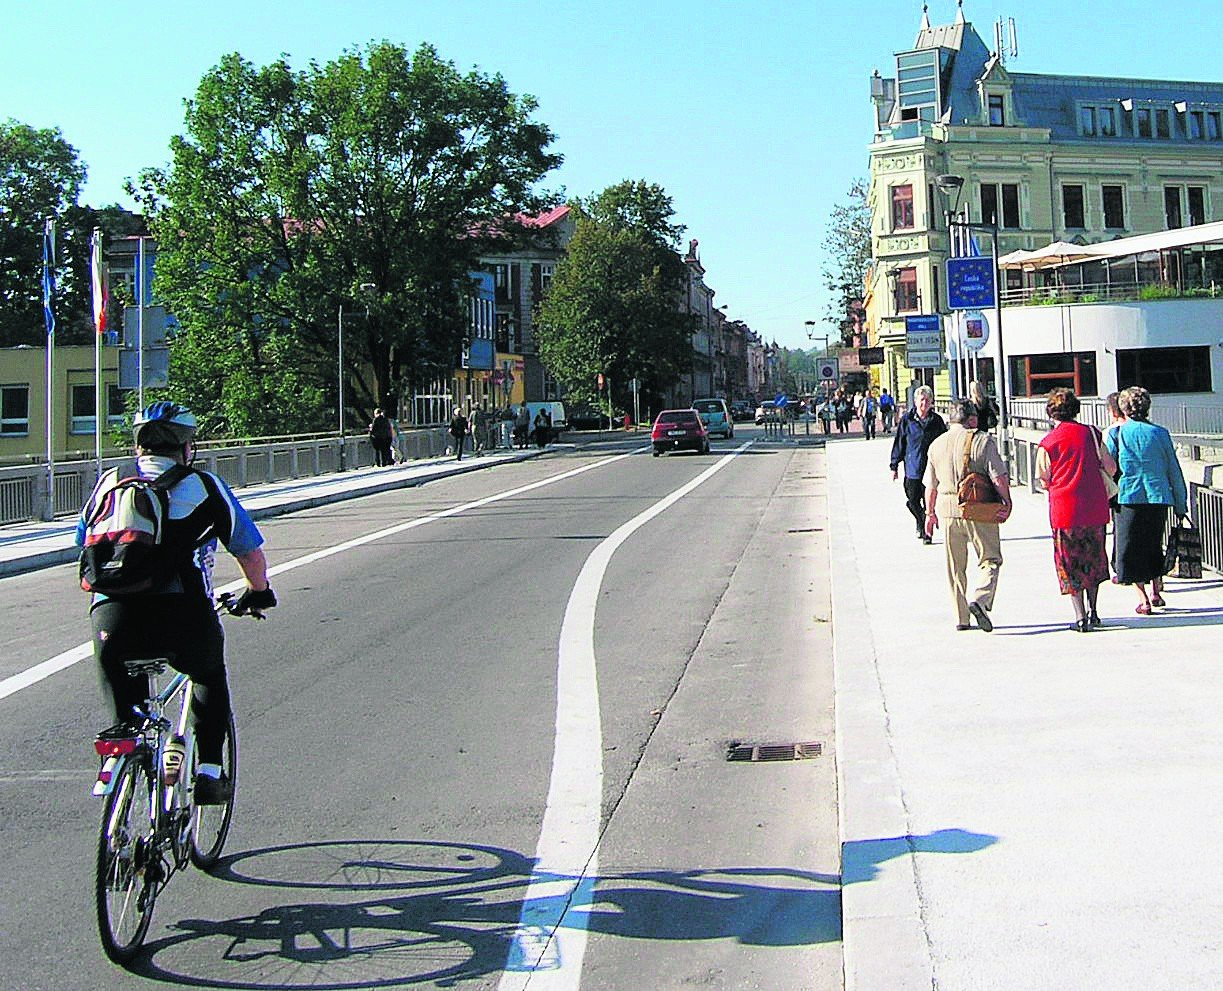
\includegraphics[scale=0.1]{4d81091f37a44_o_xlarge.jpg}}
  \end{tabular}
  %\caption{caption} %this is the caption for the whole figure delete % in front of caption if you want it.
\end{figure}
\end{frame}







\begin{comment}
\begin{frame}{Divided city of Komarom (HU) \& Komarno (SK)}
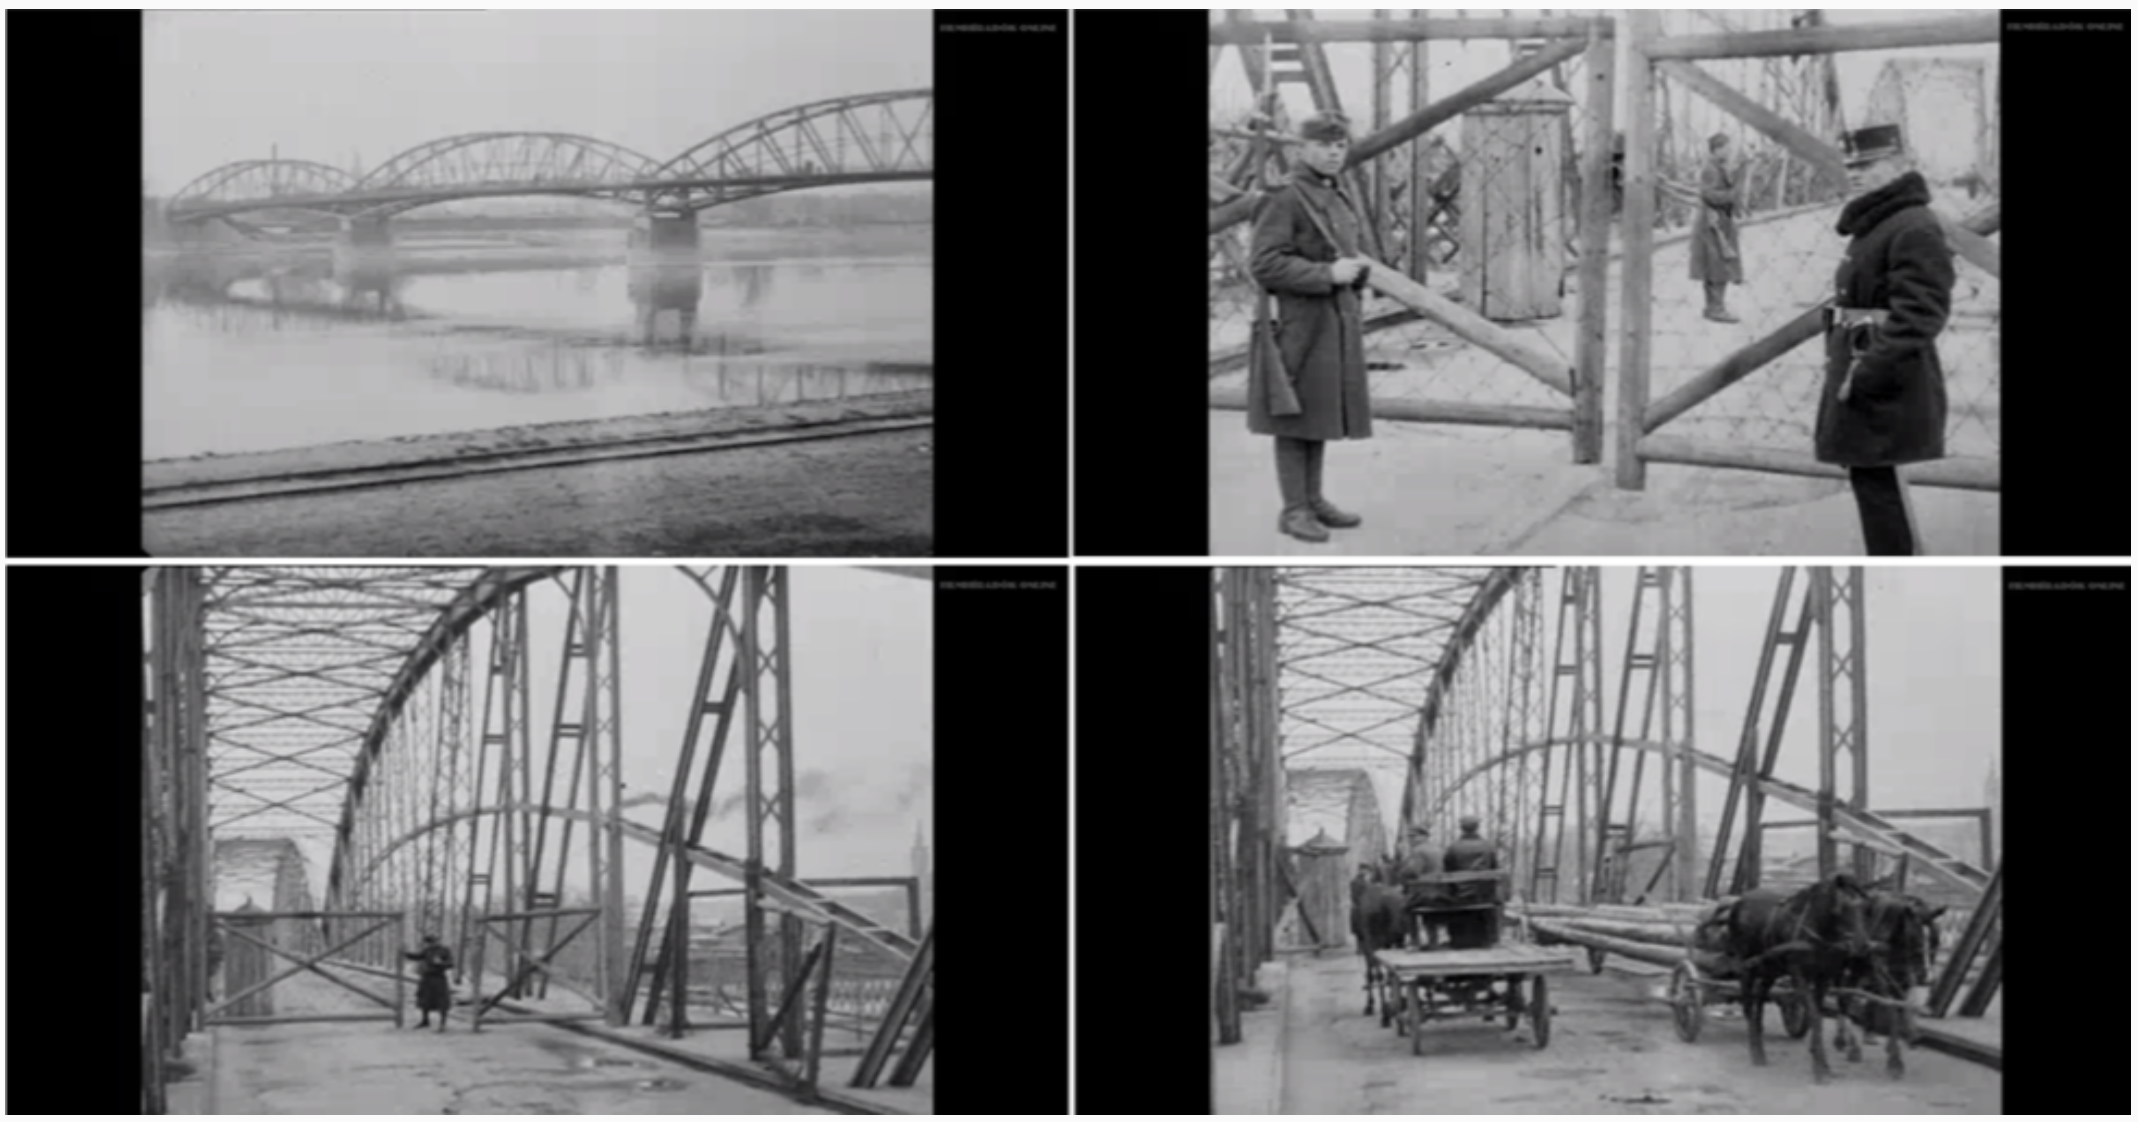
\includegraphics[scale=0.3]{HU_SK.png}
\tiny  Note: A one-minute Hungarian silent film from 1925. Photoes show border guards policing the bridge linking Komárom in Hungary with Komárno in Czechoslovakia (today in Slovakia)
\end{frame}
\end{comment}



\begin{comment}
\begin{frame}{Border Crossing between Komarom (HU) \& Komarno(SK)}
\begin{figure}
   \begin{minipage}{0.48\textwidth}
     \centering
     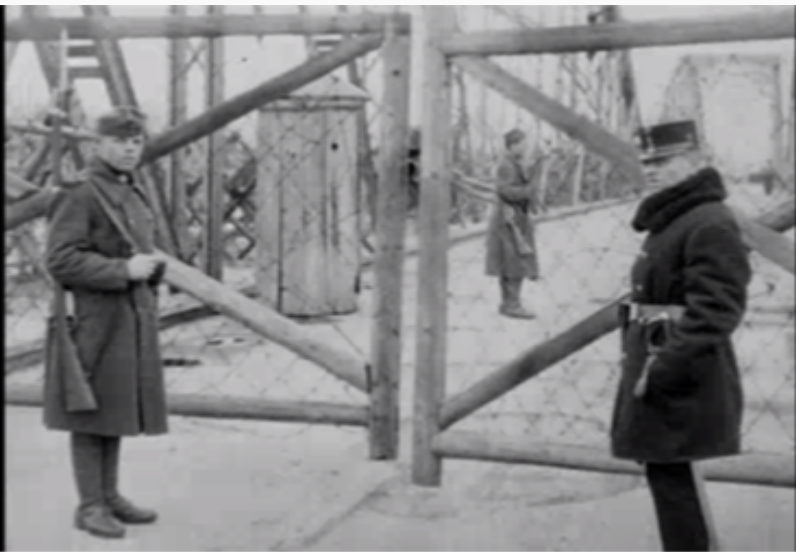
\includegraphics[width=1\linewidth]{22.png}
     \caption{\small A. Border Crossing in 1925 }
   \end{minipage}\hfill
   \begin{minipage}{0.48\textwidth}
     \centering
     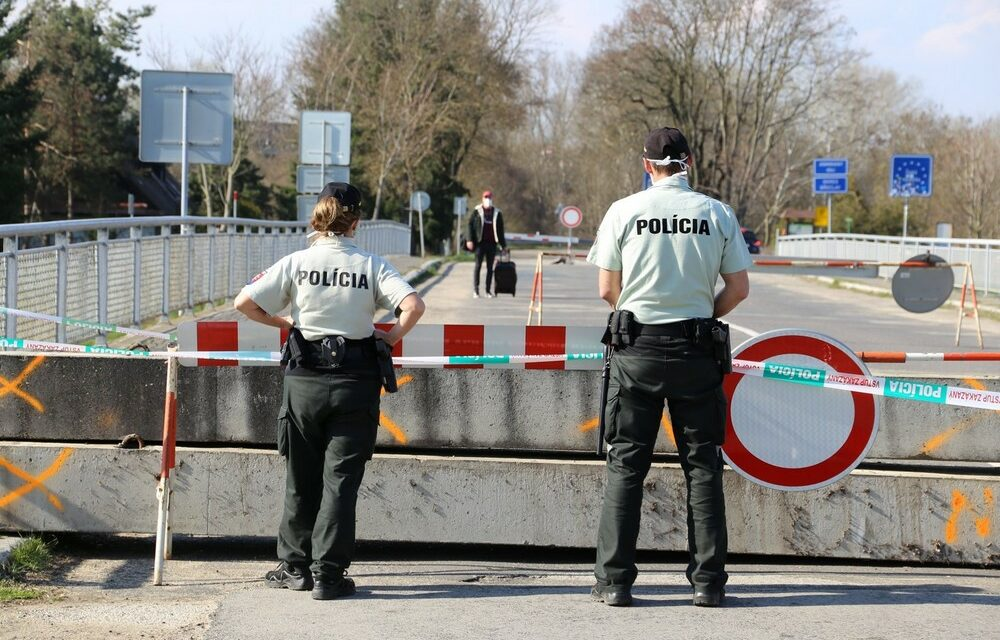
\includegraphics[width=1.1\linewidth]{33.jpg}
     \caption{\small B. Border Crossing in 2006}
   \end{minipage}
\end{figure}
\end{frame}
\end{comment}


\begin{comment}
\begin{frame}{Historical City Center: \small City Market Square in Cieszyn (PL)}
\begin{figure}[h]
\centering
\begin{tikzpicture}[spy using outlines={magnification=4, rectangle, size=3.9cm, blue, connect spies}] 
\node (n1) at (0,0){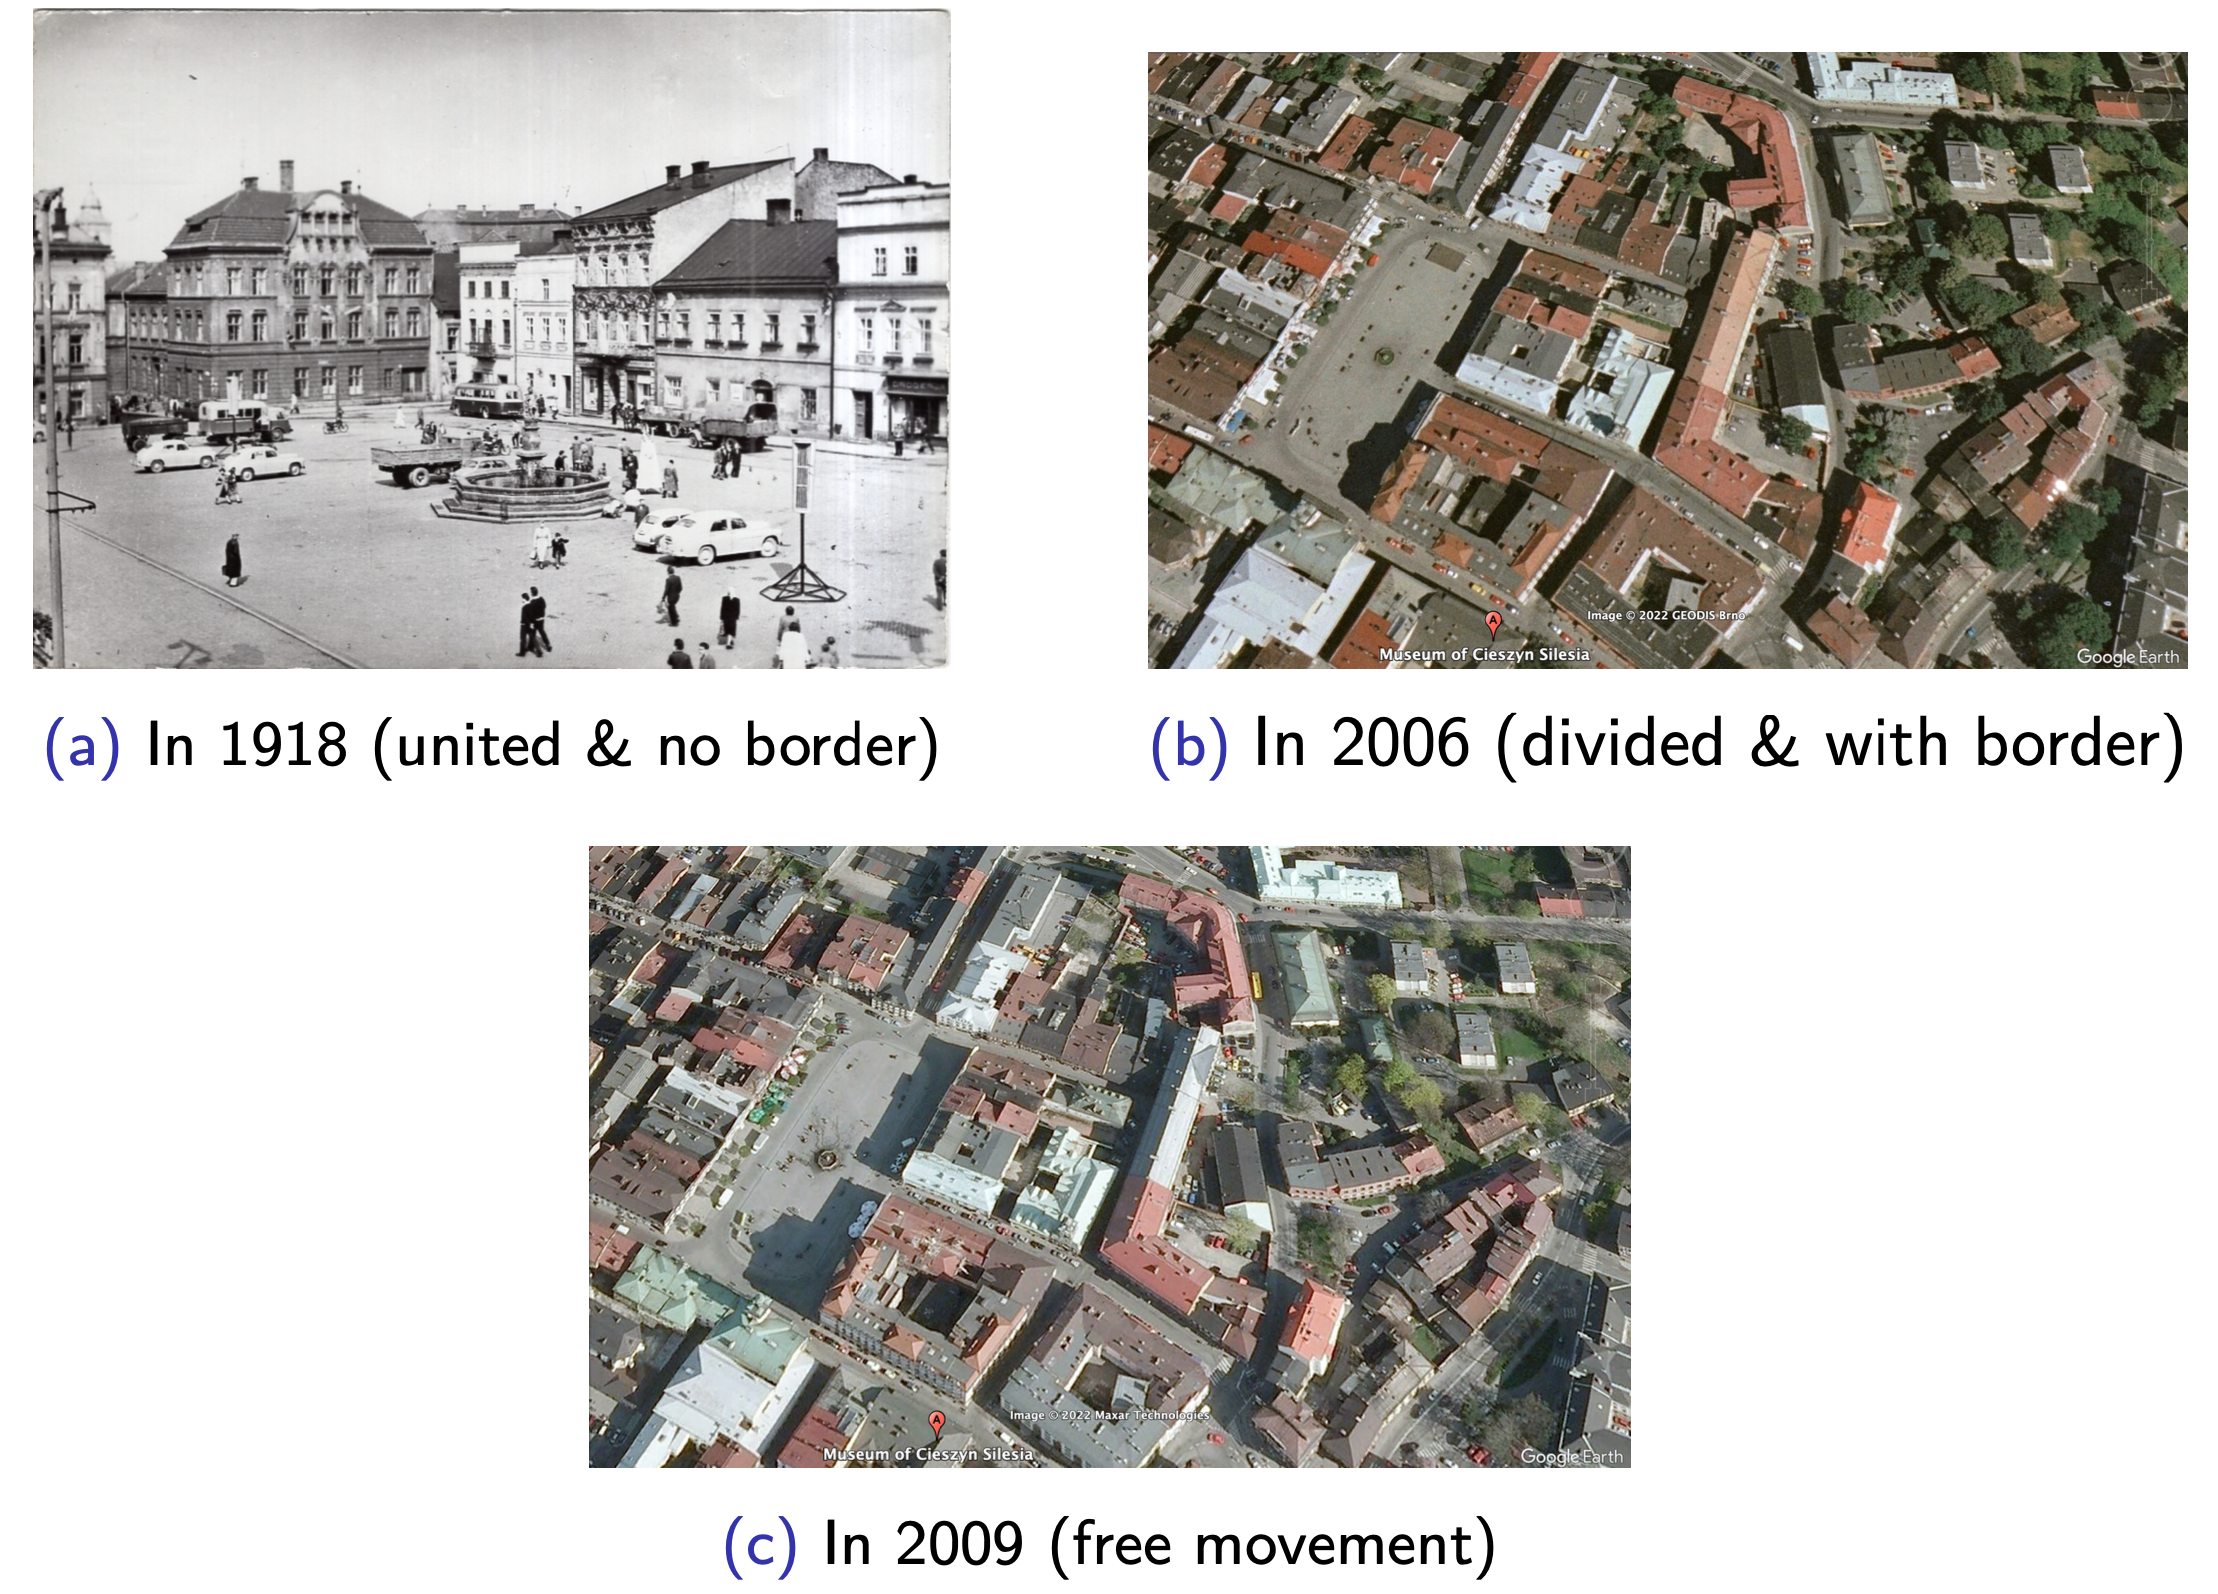
\includegraphics[scale=0.2]{fi.png}}; 
\spy on (-0.5, -1.5) in node at (-6,-3);
\spy on (1.5, 1.3) in node at (-6,1);
\end{tikzpicture}
\end{figure}   
\end{frame}
\end{comment}

\setbeamertemplate{caption}{\raggedright\insertcaption\par}
\begin{frame}{Divided Cities in Europe}
\begin{figure}
\centering
\begin{overpic}[
      width=\linewidth]{Sample1}
      \put(20,30){\hyperlink{frankfurt}{\makebox(2,2)[lb]{}}}%
       \put(38,18){\hyperlink{tesin}{\makebox(2,2)[lb]{}}}%
    \end{overpic}
\caption{ Divided Cities after the \textcolor{red}{World War II} \&  \textcolor{green}{World War I}}
\end{figure}
\end{frame}



\setbeamertemplate{caption}{\raggedright\insertcaption\par}
\begin{frame}{Three Phases: 
\\\small Pre-Division , Post-Division, and Post-Integration}
\begin{figure}
\centering
    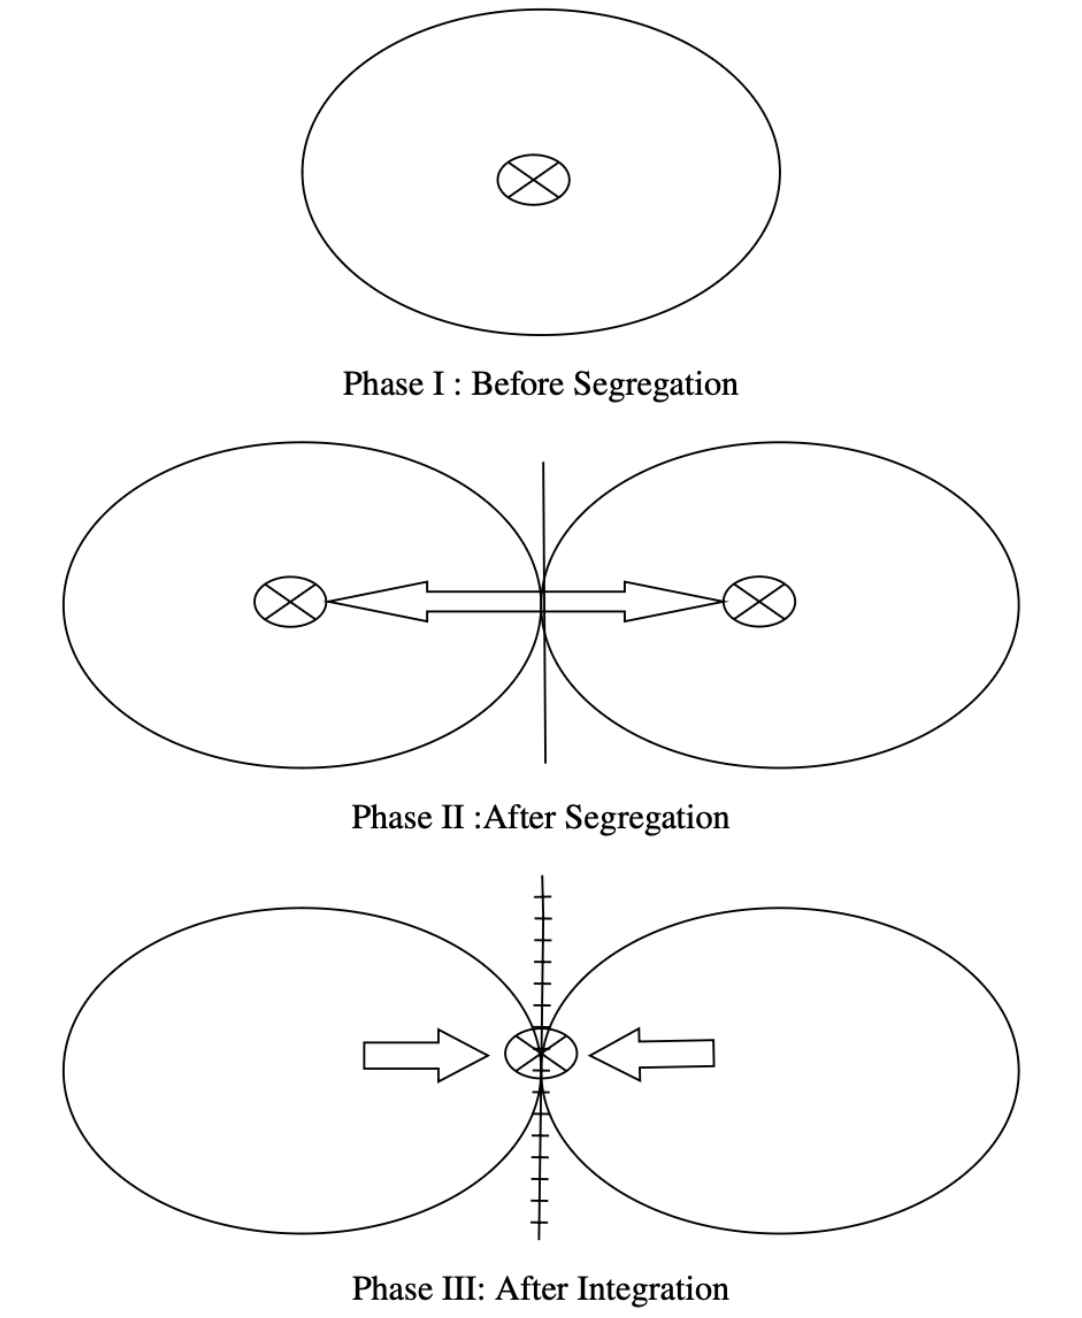
\includegraphics[scale=0.3]{hypoframe.png}
\end{figure}
\end{frame}




\begin{frame}{Preview of Main Results}
\\\textbf{} 
Following the Schengen agreements, the internal city structures of divided cities revert to their pre-division conditions. Economic activities become increasingly concentrated near former historical centers after the implementation of the free movement policy.
\vspace{0.2cm}
\justifying
\vspace{0.2cm}
\begin{itemize}
    \item \textit{Before 1990 EU integration}: Economic activities were centered away from pre-division centers. 
    \item \textit{After 2004 EU enlargment}: Economic activities remained stable.
    \item \textit{After 2008 Schengen}: Economic activity shifts to the center of the "unified city," such as pre-World War centers.
    \vspace{0.5cm}
    \item \textit{Channel I}: consumption and production oriented firms 
    \item \textit{Channel II}: cultural and language proximity 
\end{itemize}
\end{frame}








\begin{comment}
\begin{frame}{History of Study Area\\\textit{\small "One city, two states" - the motto of Valga-Valka}}
\begin{table}
\justifying
\centering
\tiny
\RawCaption{\caption{Borders in Divided Cities}}
\vskip\captionskip
    {}
{
\def\sym#1{\ifmmode^{#1}\else\(^{#1}\)\fi}
\noindent\makebox[\linewidth]{
\begin{tabular}{|l|l|l|l|}
\hline
\textbf{}  \textbf{Divided City (A)}& \textbf{Divided City (B) }              &\textbf{Rise \& Fall}   & \textbf{Pre-division Centers}\\                                          
\hline
\hline
   Frankfurt (Oder) (DE)                                           & 
  Słubice (PL) & 1945 \& 2008                   
                  &    Museum Viadrina (DE)\\
                  \hline
                                   Görlitz (DE)                                                     & Zgorzelec (PL)
                & 1945 \& 2008 &  Historical Museum (DE) \\
\hline
                     Guben (DE)                                                       & Gubin (PL)         &1945 \& 2008                             &  City Museum (DE)\\
\hline
              Bad Muskau (DE)                                                 & Łęknica (PL)  & 1945 \& 2008                &   Schloßvorwerk (DE) \\ 
\hline
                    Gorizia (IT)                                                      & Nova Goricia (SI)    
 
 & 1945 \& 2008  & Palazzo Lantieri (IT)\\
\hline
          Bad Radkersburg (AT)                                            & 
  Gornja
  Radgona (SI)
       &  1920 \& 2008               &  Frauenkirche  (DE)\\
\hline
                   Komarom (HU)                                                    & Komarno (SK)                      & 1920 \& 2008                &   György Klapka Museum (HU) \\
 \hline
            Sátoraljaújhely (HU)                                            & 
  Slovenské
  Nové Mesto (SK)
   & 1920 \& 2008            &   Kazinczy Múzeum (HU)\\
\hline
                    Cieszyn (PL)                                                     & Český Těšín (CZ)               & 1920 \& 2008                  &  Museum of Cieszyn (PL)\\

         \hline
                     Gmünd (AT)                                                      & České Velenice (CZ)                & 1920 \& 2008             &   Schloss (Castle) Gmünd (AT)\\
 
   \hline
                       Valka (LV)                                                       & Valga (EE)                         & 1920 \& 2008   & Valga Museum (EE)
 \\
\hline
 \end{tabular} 
 }}
\end{table}
\end{frame}
\end{comment}


\begin{comment}
\begin{frame}{Theoretical Predictions I \\\small Hypotheses}
    \begin{itemize}
    \justifying
        \item \textbf{\textit{Hypothesis I:}} Economic activities become denser near pre-division historical centers than in other zones after 2008.
        \vspace{0.2cm}
        \end{itemize}
\textit{This raises an important question:} what type of border opening is more important in spurring agglomeration, the free movement of goods or of people?
When looking into potential mechanisms behind the impact I hypotheses the following: 
       
\end{frame}








\begin{frame}{Theoretical Predictions II \\\small Hypotheses}
    

\textbf{\textit{Hypothesis IIa:}} Newly established economic entities are highly concentrated near pre-division historical centers after free movement of people was allowed - after 2008.
         \vspace{0.2cm}
         \item \textbf{\textit{Hypothesis IIb:}} Newly established economic entities are not concentrated near pre-division historical centers after broader market access was established - after 2004.
        \vspace{0.2cm}
        \item \textbf{\textit{Hypothesis III:}} After division, newly established economic entities were highly concentrated away from pre-war historical centers between 1945 and 1990.
    
\end{frame}



\begin{frame}{Three Stages of Theoretical Framework}
\centering
    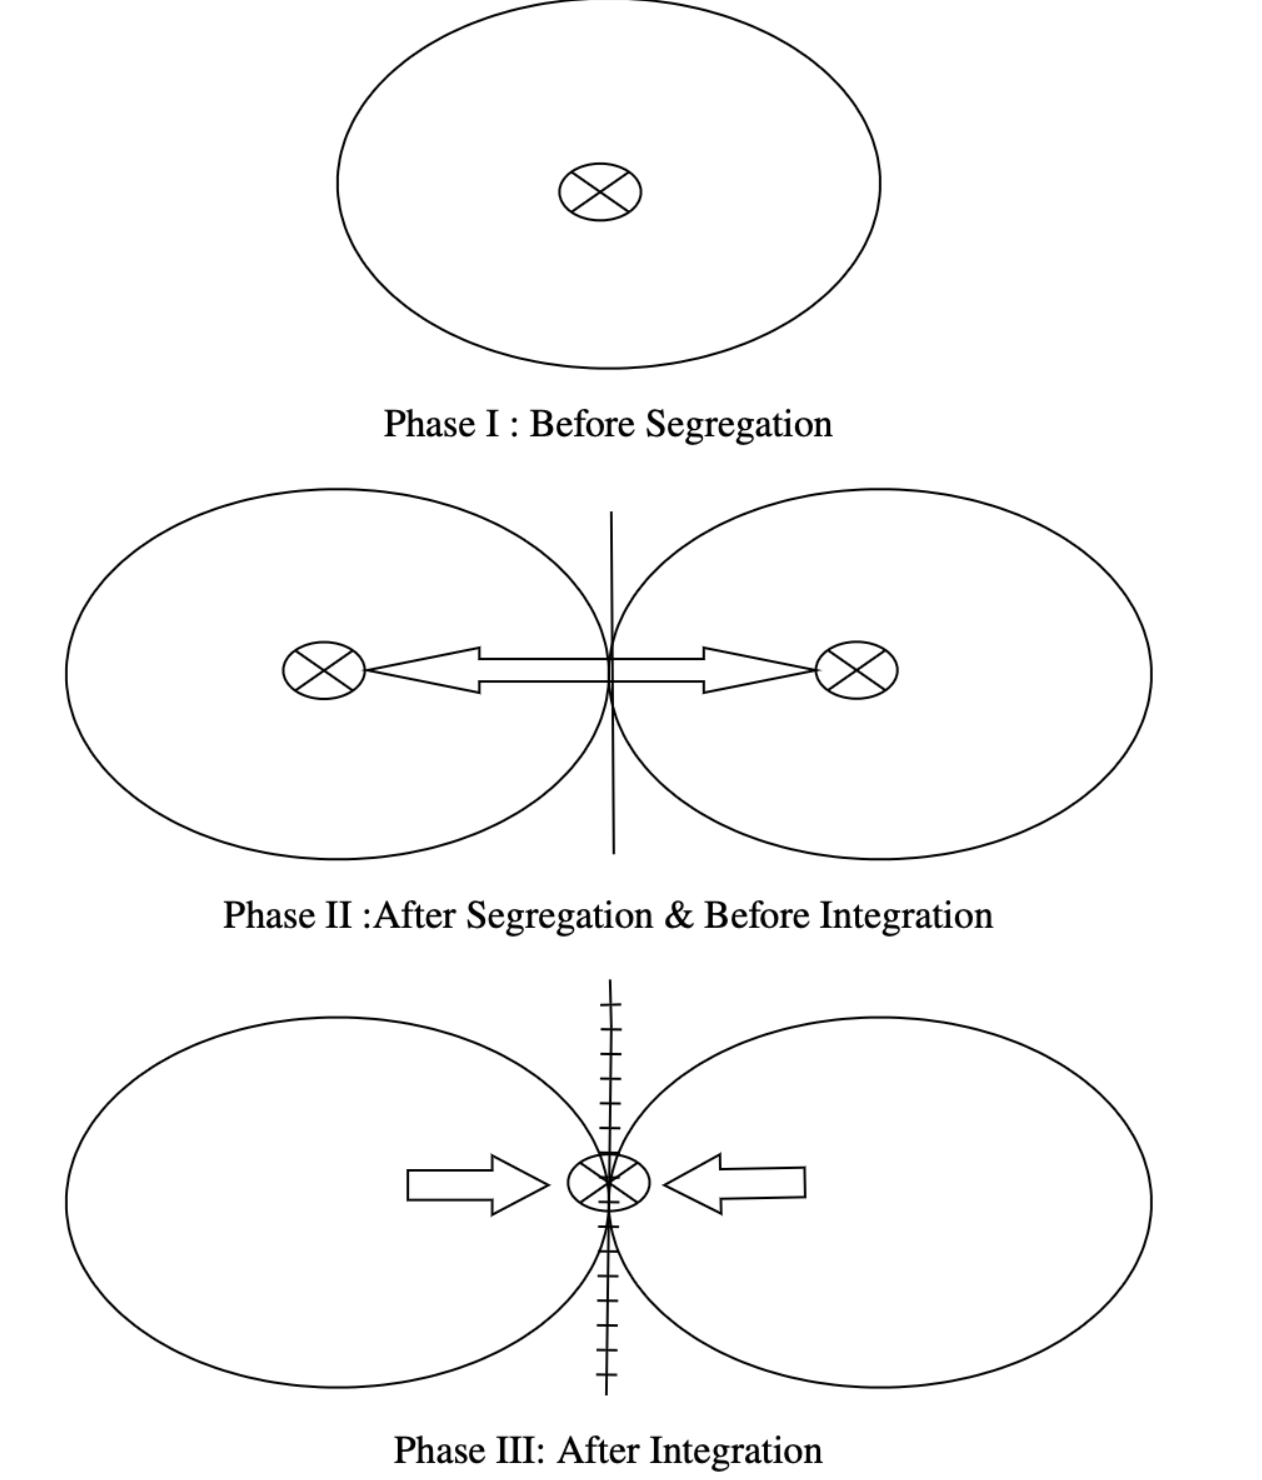
\includegraphics[scale=0.3]{kk.png}
\end{frame}
\end{comment}








\begin{frame}{Data \\\small Unconventional \& Conventional Datasets}
Data I: Nighttime Lights
\begin{itemize}
    \item The Defense Meteorological Satellite Program (DMSP) 
    \item Time span:  1992-2013 
    \item Resolution scale 1x1 $km^{2}$
    \item Digital numbers (DN) ranges 0-63
    \item 3400 pixels over 22 years 
$\approx$ 74,729 pixels
    %\item \textit{satellite errors random}: averaged data from two satellites
    %\item \textit{satellite errors are not random}: included satellite fixed effects in the model
     \end{itemize}
 \end{frame}

\begin{comment}
\begin{frame}{Night lights in Europe}
\centering

\includegraphics[scale=0.35]{DividedCities_pres/1992.png}
\end{frame}


\begin{frame}{Night lights in Europe}
\centering

\includegraphics[scale=0.35]{DividedCities_pres/2010.png}
\end{frame}
\end{comment}


\begin{frame}{Data \\\small Unconventional \& Conventional Datasets}
\\Data II: Registers of Economic Entities
\begin{itemize}
\item Statistical Offices and Ministry of Justice's Information Service: Hungary, Czech Republic, Slovakia 
\item Archives, Agency of Legal Records (AJPES): Slovenia
\item Business data, Digital Database of Companies (AIDA): Italy
\item Web Scraping at Common Registers Portals: Germany, Poland, Latvia, Estonia 
 \end{itemize}
 \end{frame}
    





\begin{frame}{Nightlights in 2002}
\begin{figure}
\justifying
\begin{itemize}
Frankfurt (Oder) - Słubice
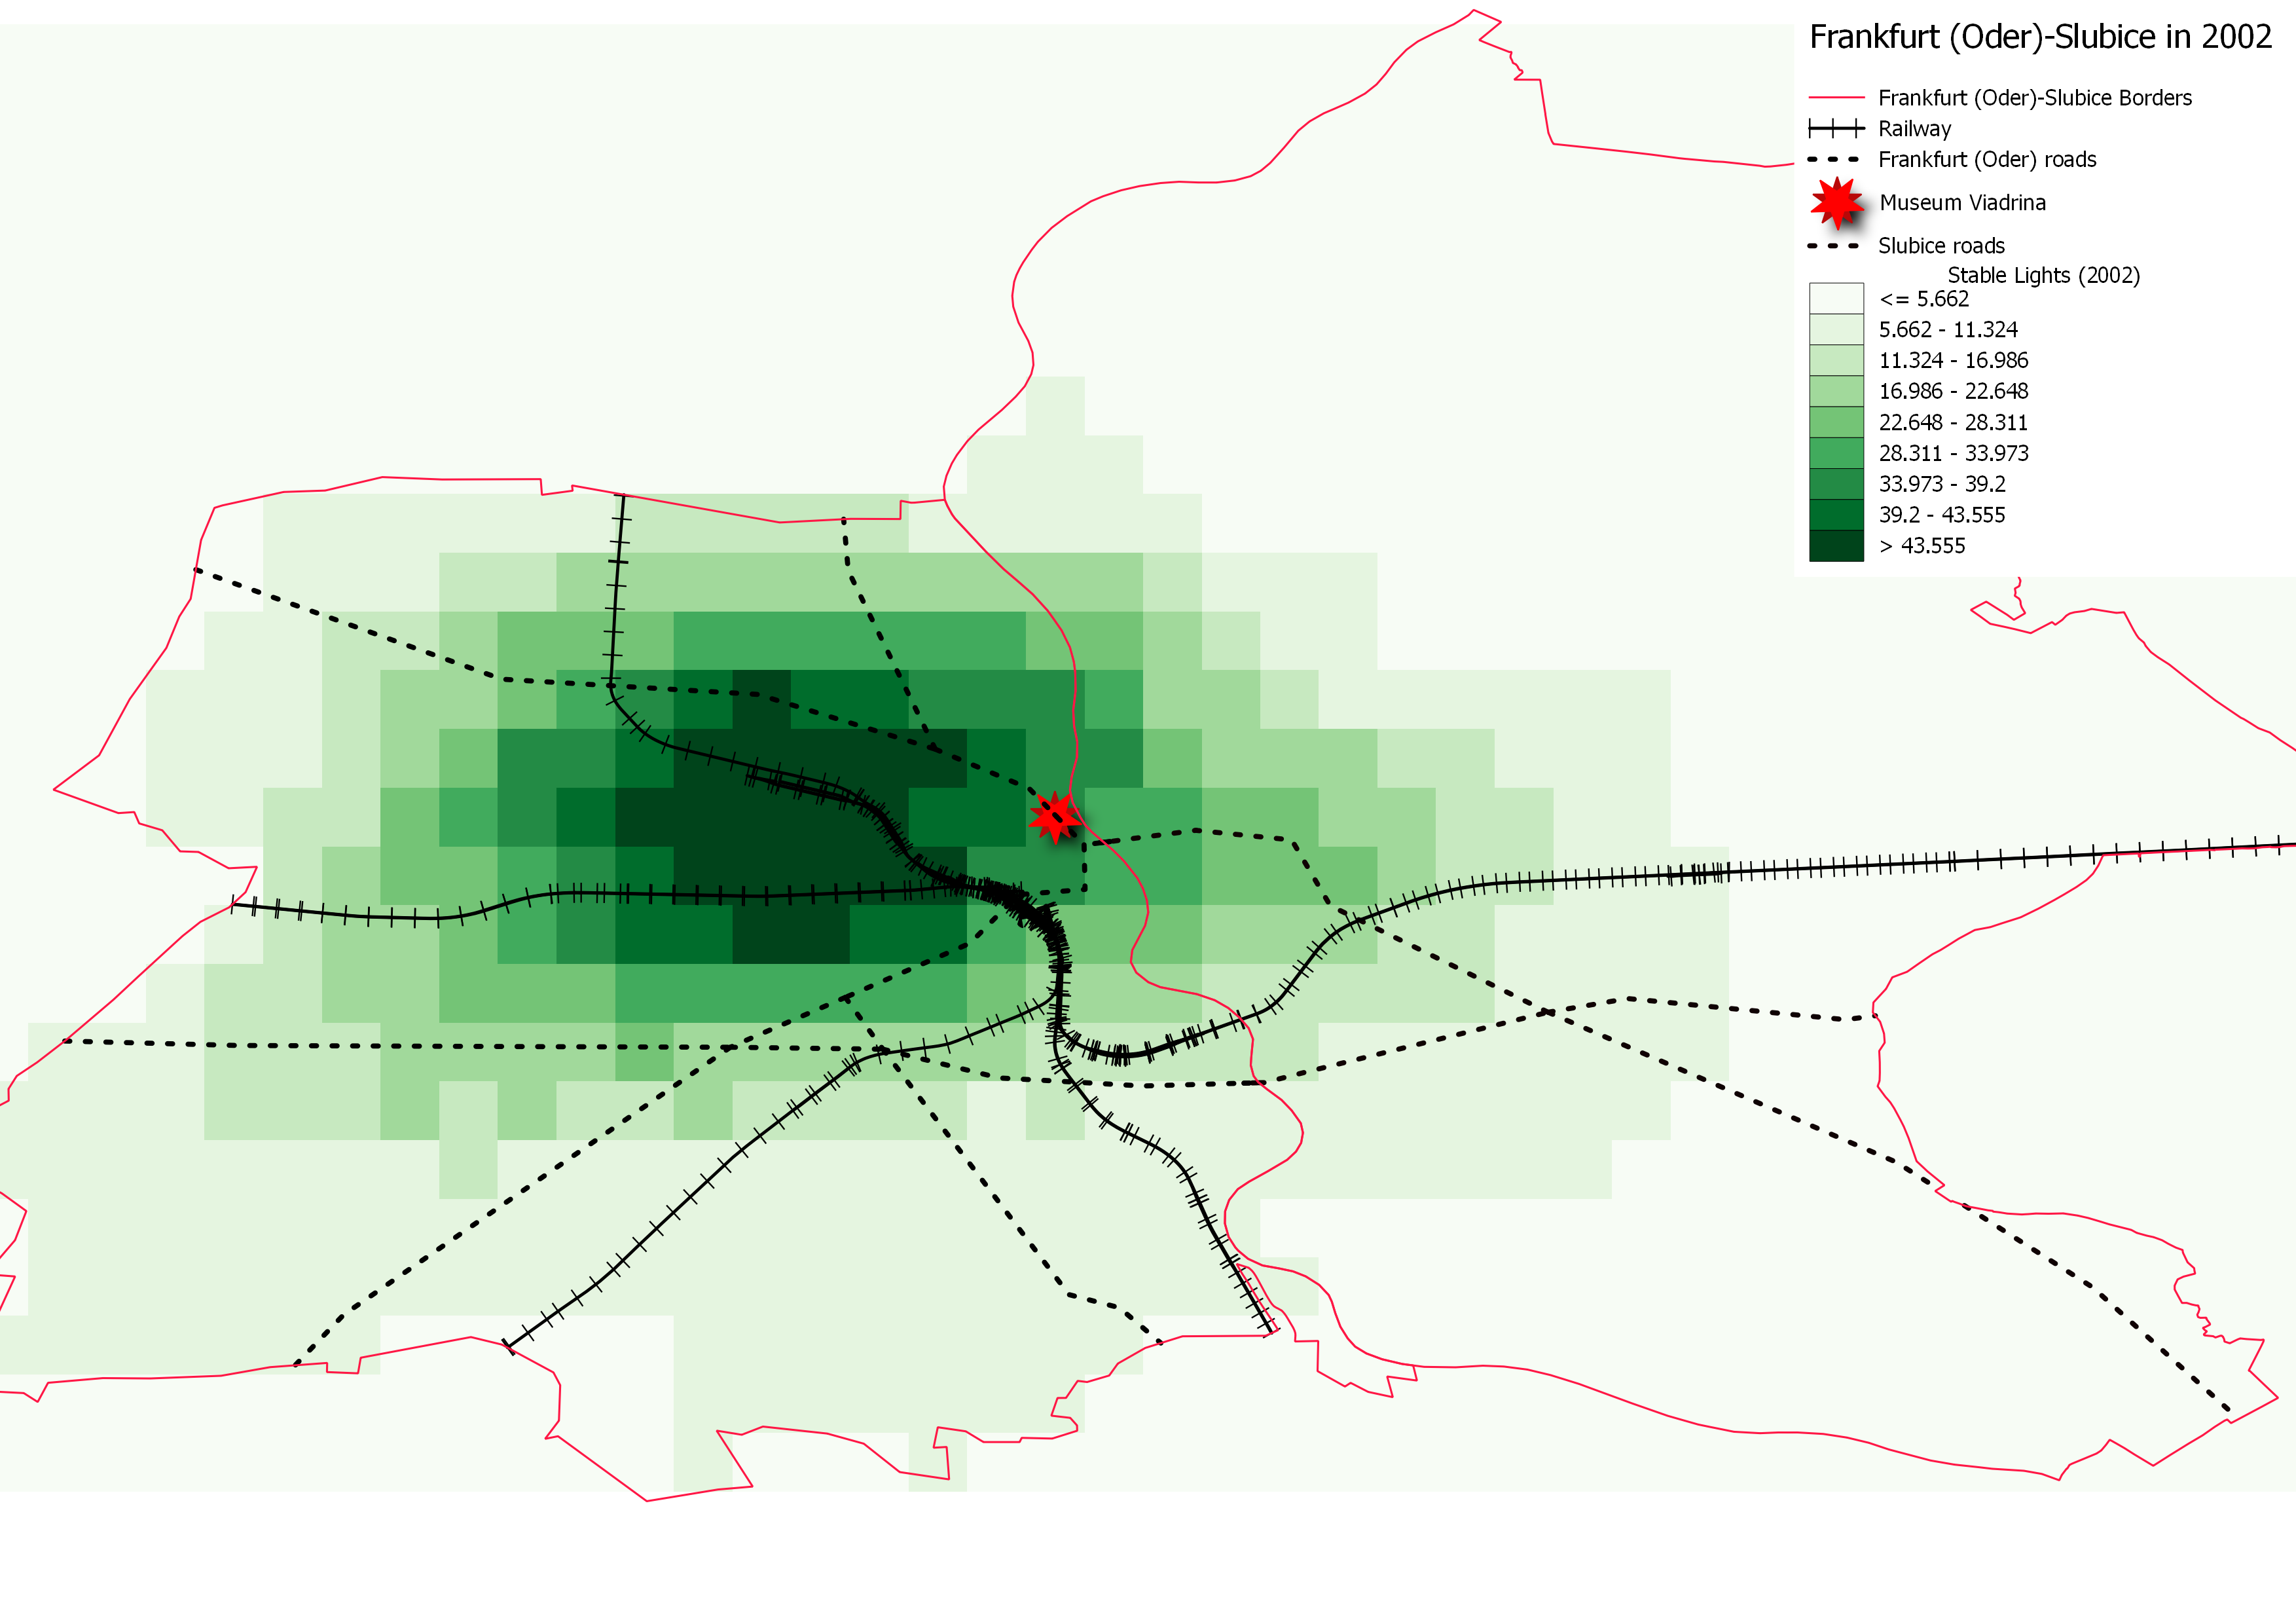
\includegraphics[scale=0.3]{FS2002.png}
\end{itemize}
\end{figure}
\end{frame}
\begin{frame}{Nightlights in 2008}
\begin{figure}
\justifying
Frankfurt (Oder) - Słubice
\begin{itemize}
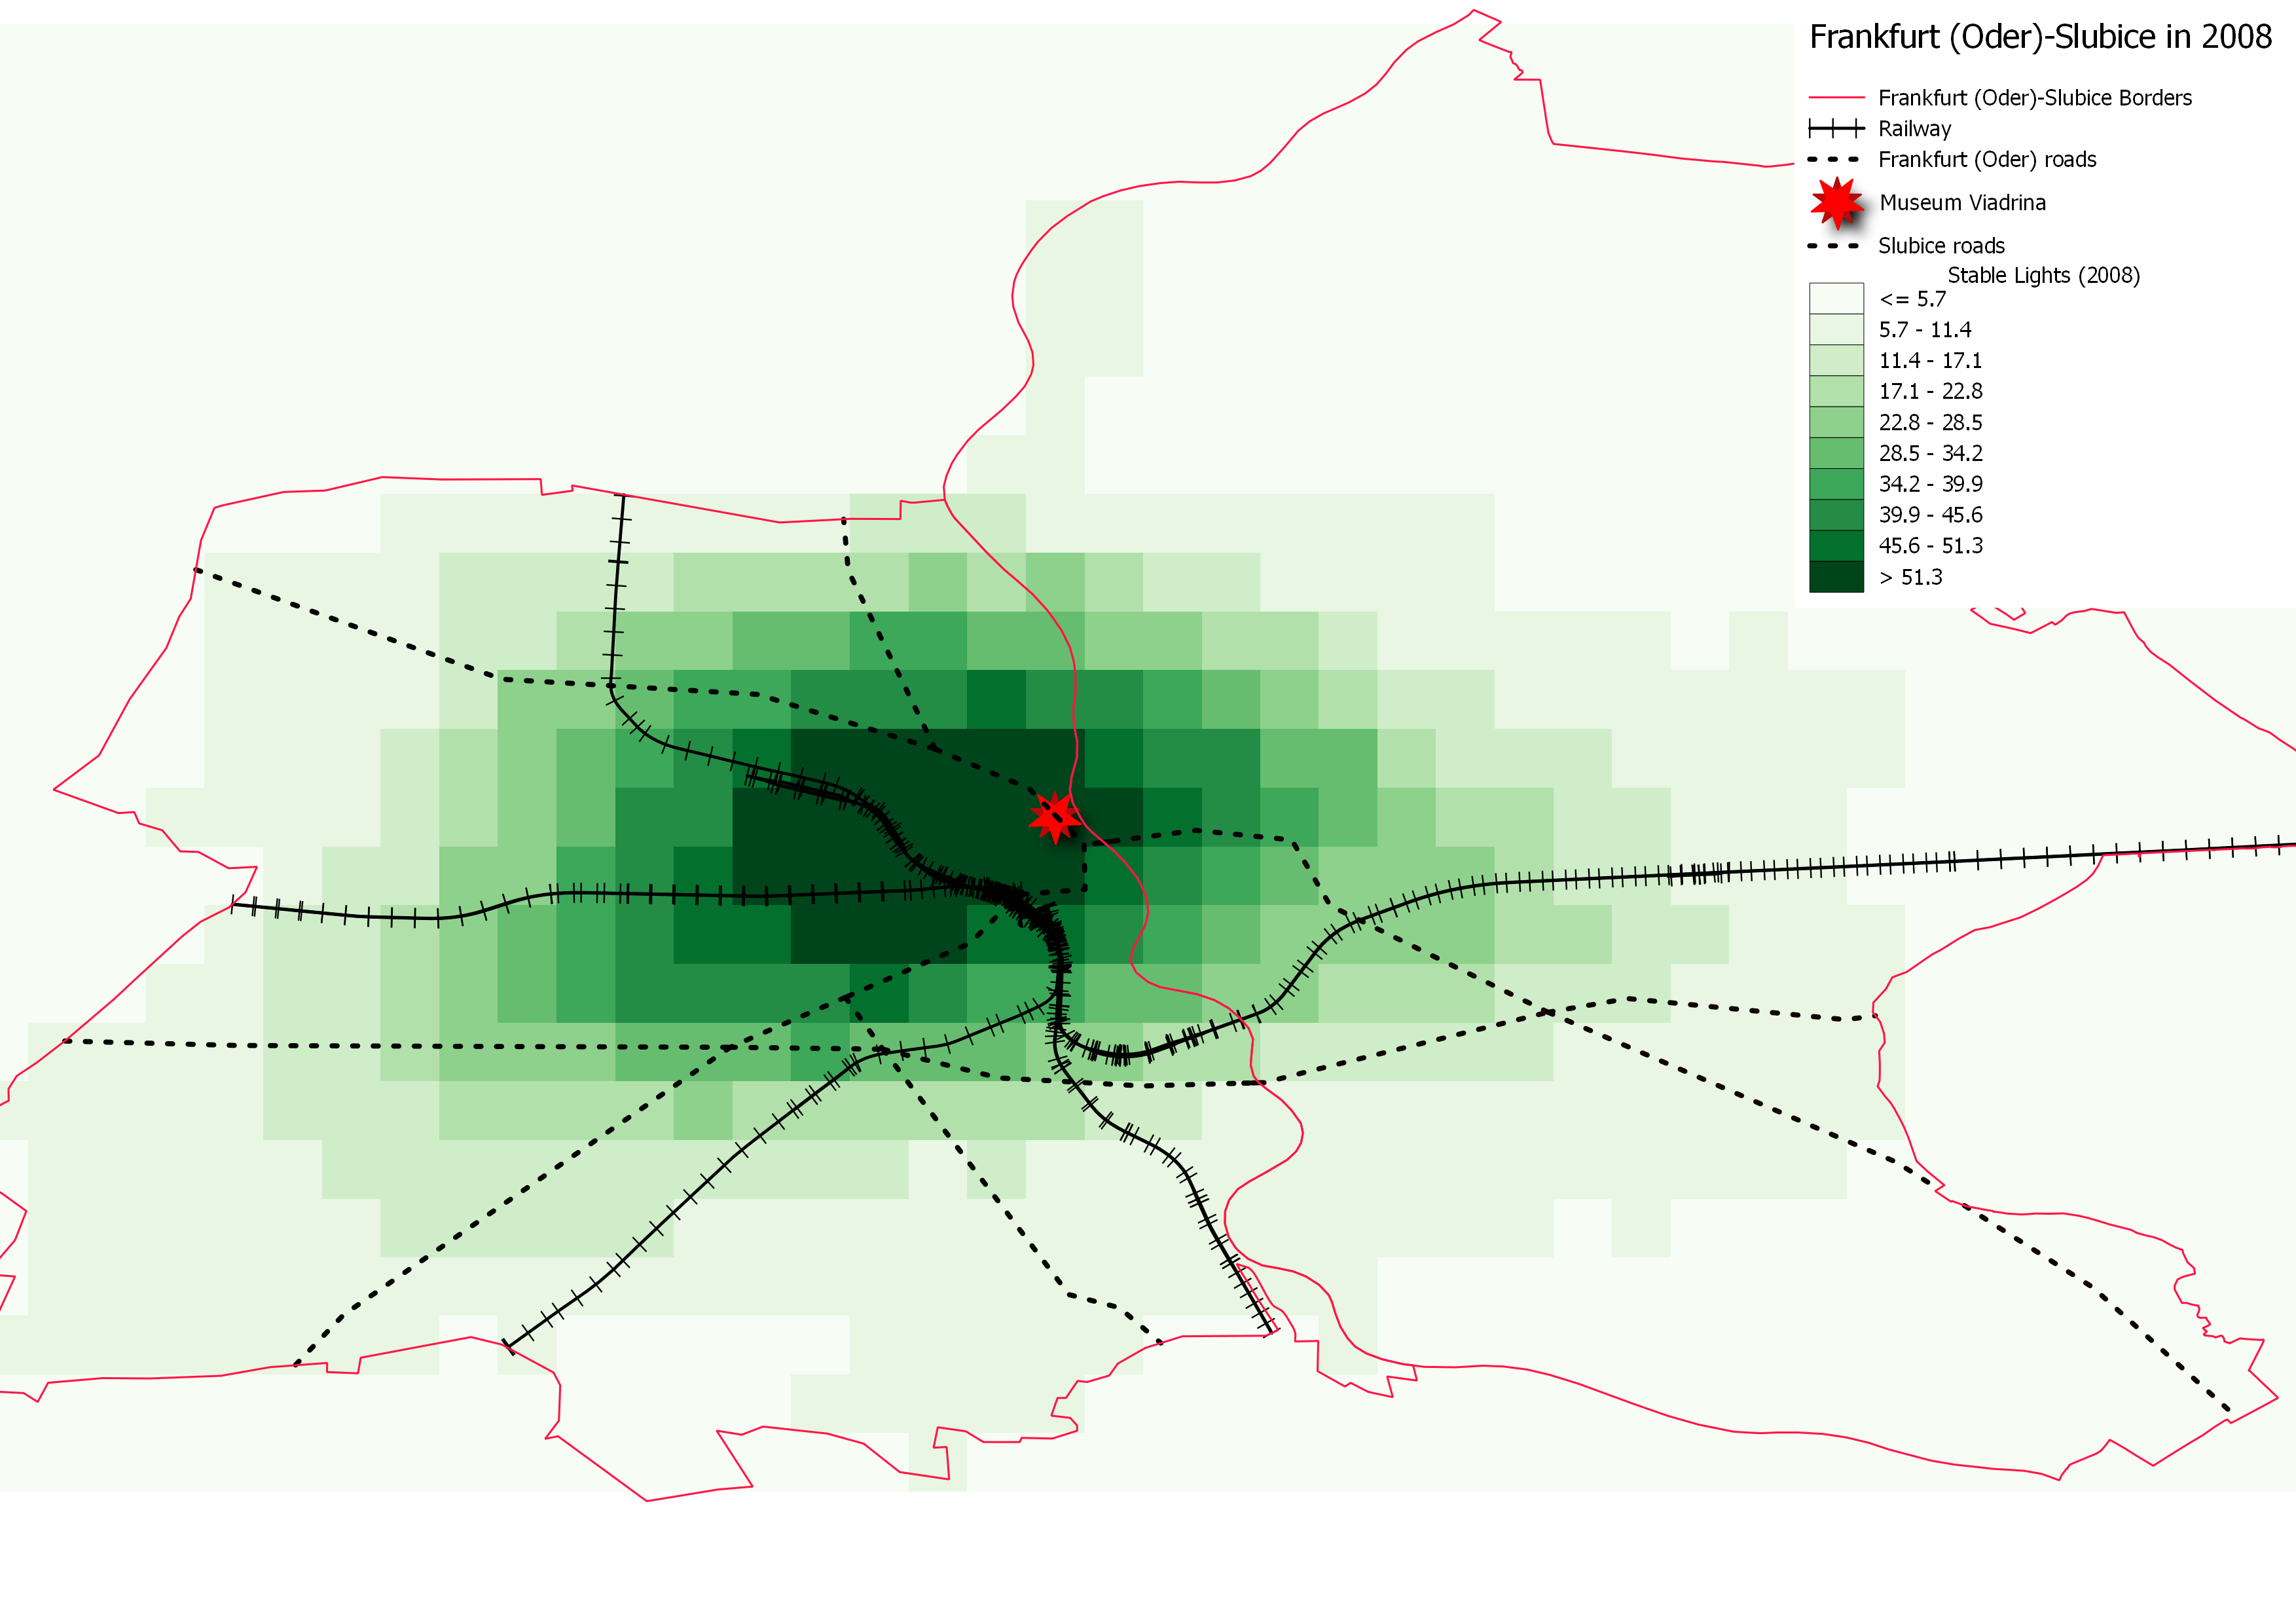
\includegraphics[scale=0.3]{FS2008.png}
\end{itemize}
\end{figure}
\end{frame}

\begin{frame}{ Nightlights in 2012}
\begin{figure}
Frankfurt (Oder) - Słubice
\justifying
\begin{itemize}
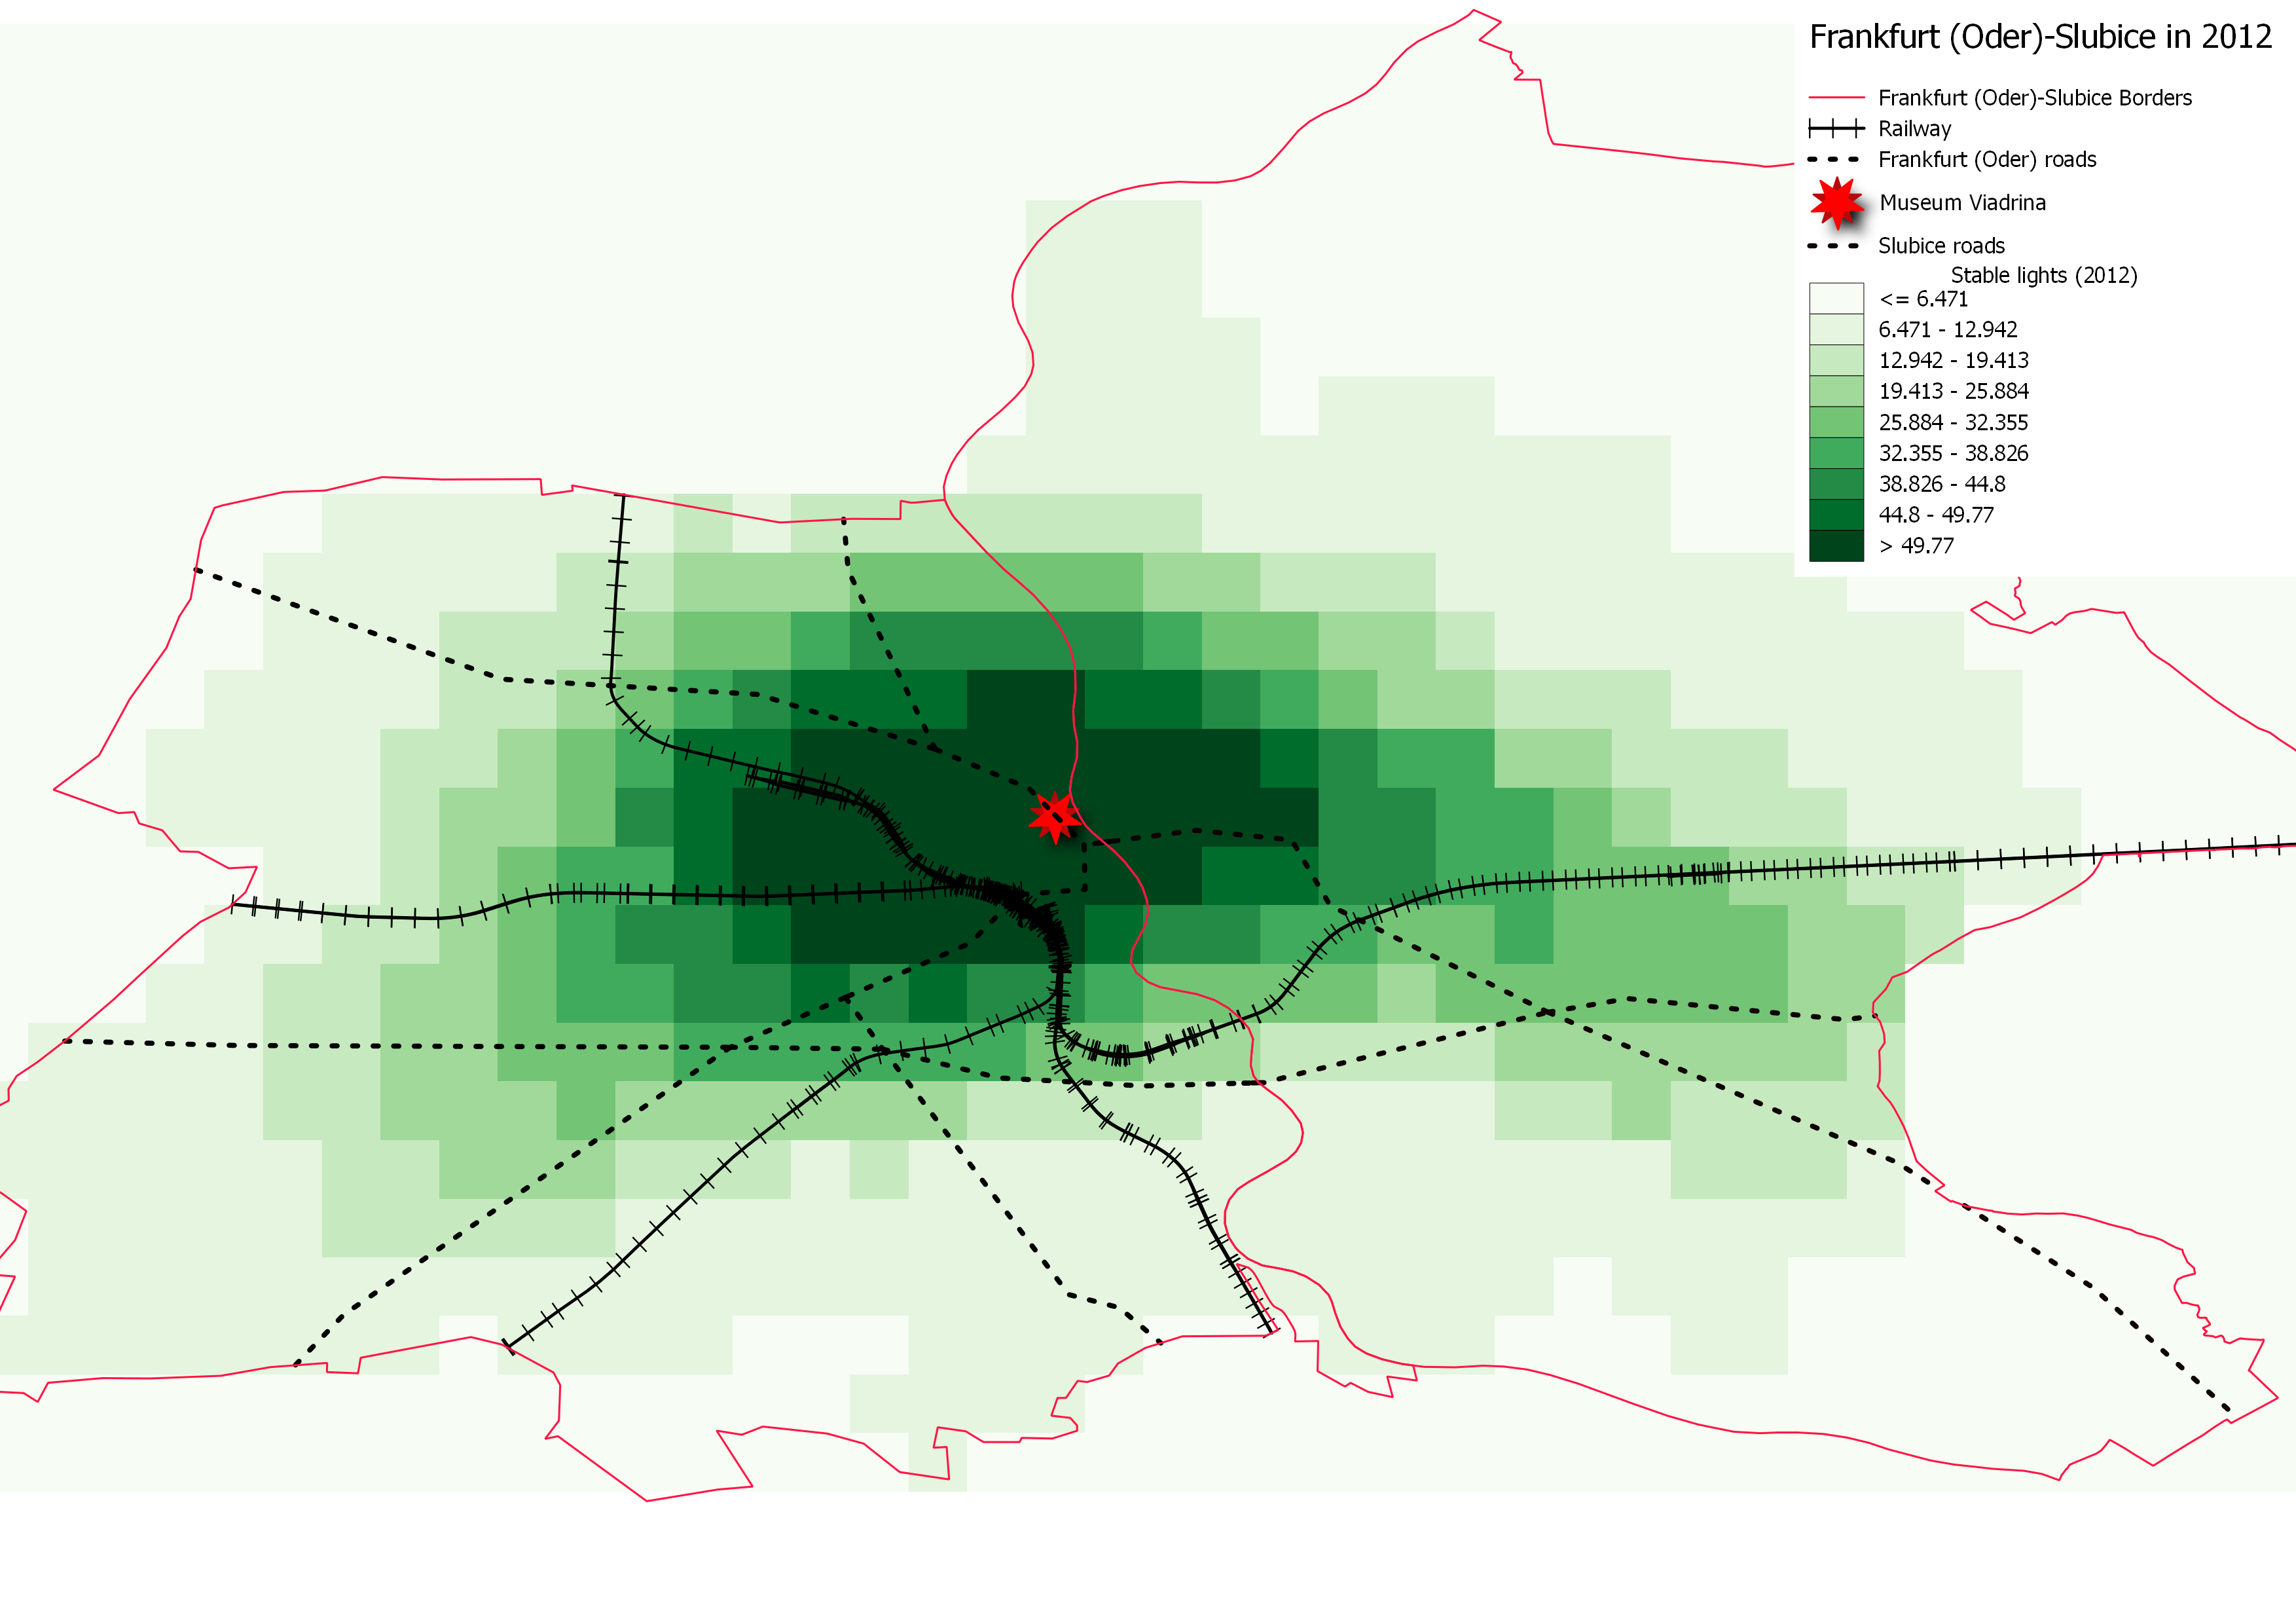
\includegraphics[scale=0.3]{FS2012.png}
\end{itemize}
\end{figure}
\end{frame}


\begin{comment}
\begin{frame}{Data I: Satellite DMSP-OLS}
\begin{figure}
\justifying
\begin{itemize}
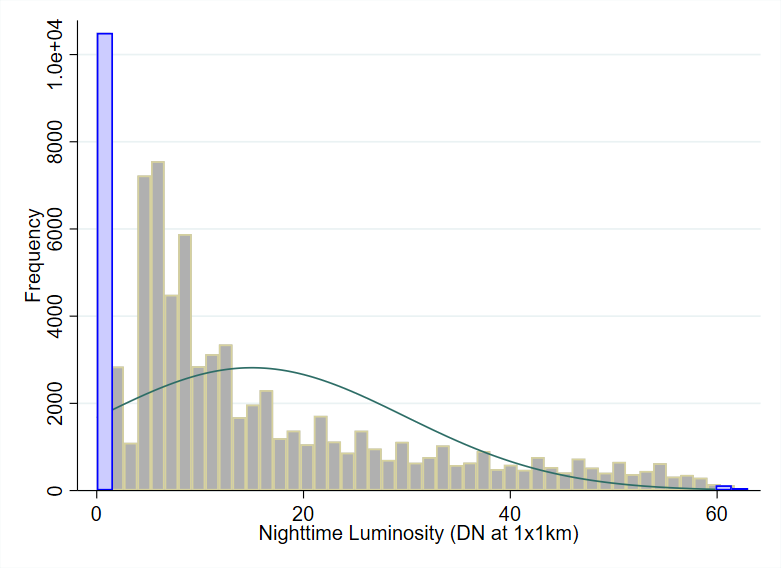
\includegraphics[scale=0.35]{predata1.png}
\end{itemize}
\end{figure}
\end{frame}
\end{comment}




    


 \begin{frame}{Collected Data }
\scriptsize
    \begin{table}[H]\centering \caption{Registered Economic Entities in Divided Cities \label{descstat}}
\begin{tabular}{|ll|lll|l|}
\hline
\textbf{City}  & \textbf{Country} & \textbf{Entry Date} & \textbf{NACE} & \textbf{Lat-Long}  & \textbf{N} \\
\hline
\hline
Cieszyn        & Poland           & Y                       & Y        & Y   & 6710     \\

Cesky Tesin    & Czechia          & Y                      & Y        & Y   &4387     \\
\hline
Komarom        & Hungary          & Y                      & Y        & Y      & 998  \\

Komarno        & Slovakia         & Y                       & Y        & Y   & 19354     \\
\hline
Nova Gorica    & Slovenia         & Y                     & Y        & Y    &  7903    \\

Goriza         & Italy            & Y            & Y            & Y          &  1002     \\
\hline
Valga          & Estonia          & Y            & Y           & Y            &650   \\

Valka          & Latvia           & Y            & N            & Y            & 540    \\
\hline
Slubice        & Poland           & Y            & Y           & Y             & 5554 \\

Frankfurt      & Germany          & Y            & N            & Y           & 2035    \\
\hline
Gubin          & Poland           & Y            & Y           & Y          & 458    \\

Guben          & Germany          & Y             & N            & Y           & 640     \\
\hline
Zhorlec        & Poland           & Y            & Y           & Y         &2695      \\

Gorlitz        & Germany          & Y             & N            & Y            & 1743     \\
\hline
Ceske Velenice & Czechia          & Y            & Y           & Y     & 738    \\

Gmund          & Austria          & N             & N            & N         & -    
 \\
\hline
\hline
Total          &           &                         &          &   & 54,669   \\
\hline
\end{tabular}
\end{table}

\end{frame}
    
    

\begin{frame}{\small Geo-referenced Economic Entities in Český Těšín (CZ) and Cieszyn (PL)}
\begin{figure}
\justifying
\begin{itemize}
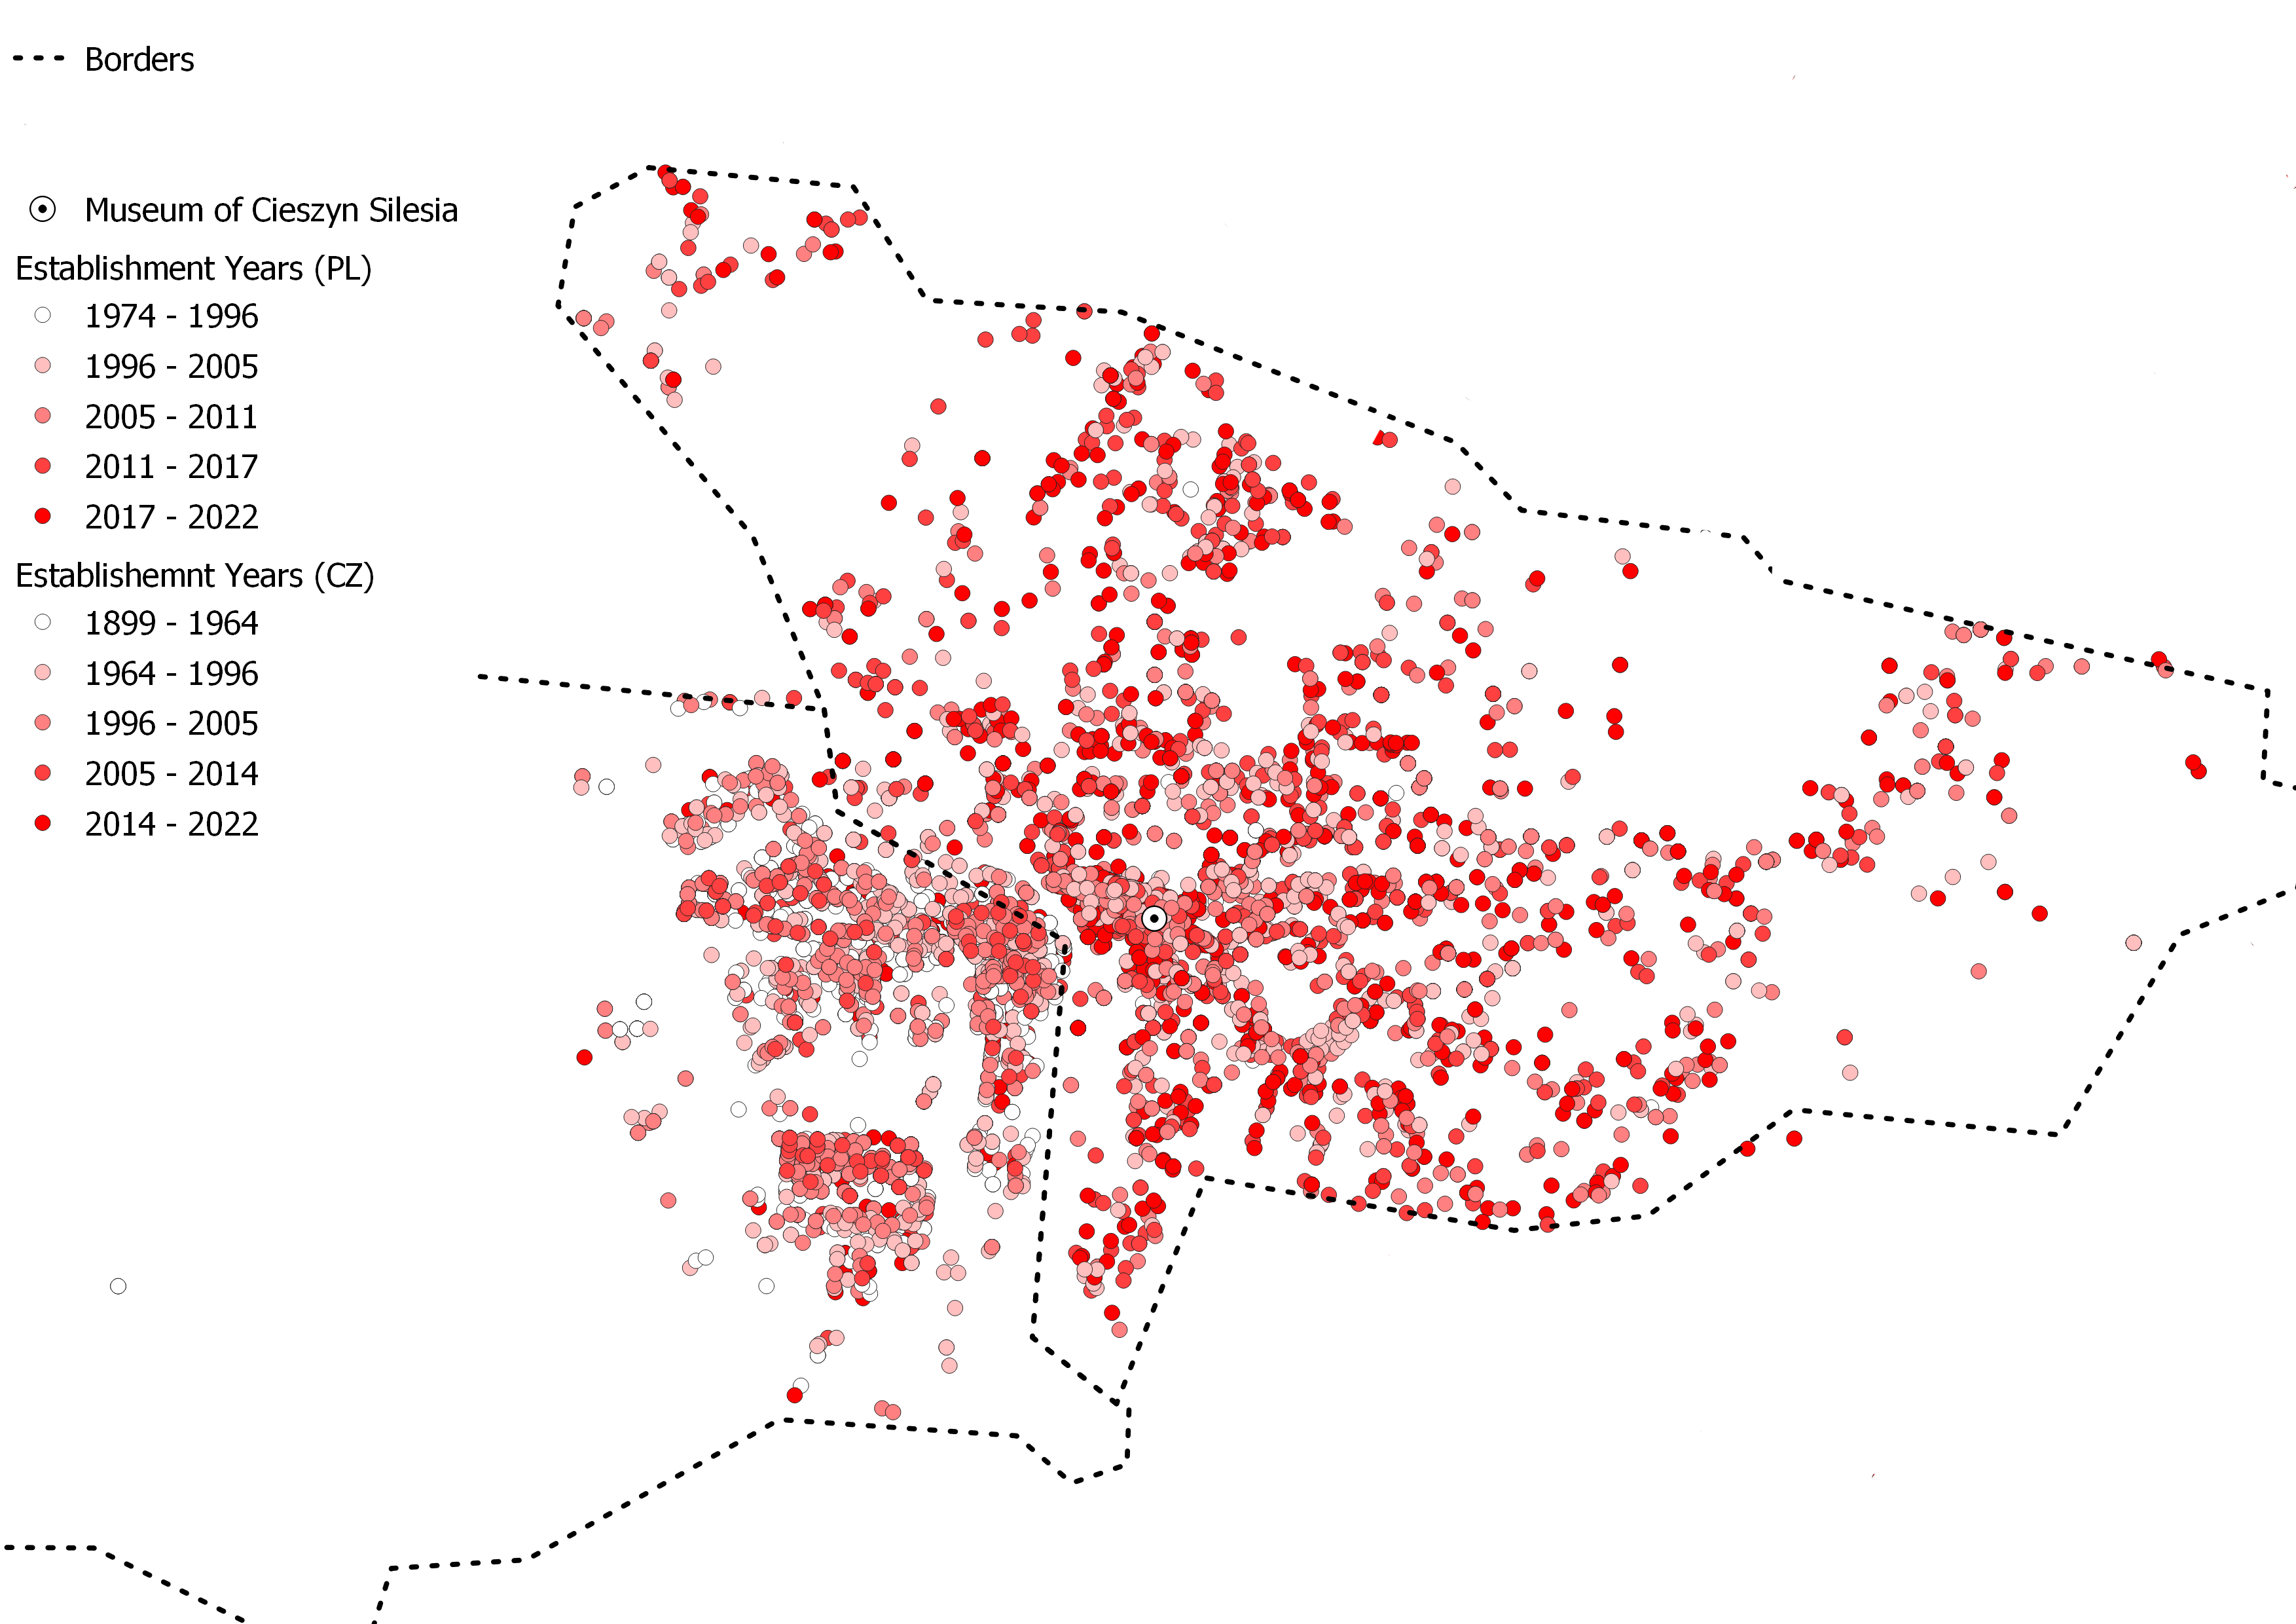
\includegraphics[scale=0.35]{cz_pl.png}
\end{itemize}
\end{figure}
\end{frame}


\begin{frame}{\small Result I
\\ Nightlights in Divided Cities: Assessing the Impact of Stepwise Integration}
\justifying
\centering
\small Economic activities become increasingly concentrated near former historical centers after the implementation of the free movement policy.
\begin{figure}
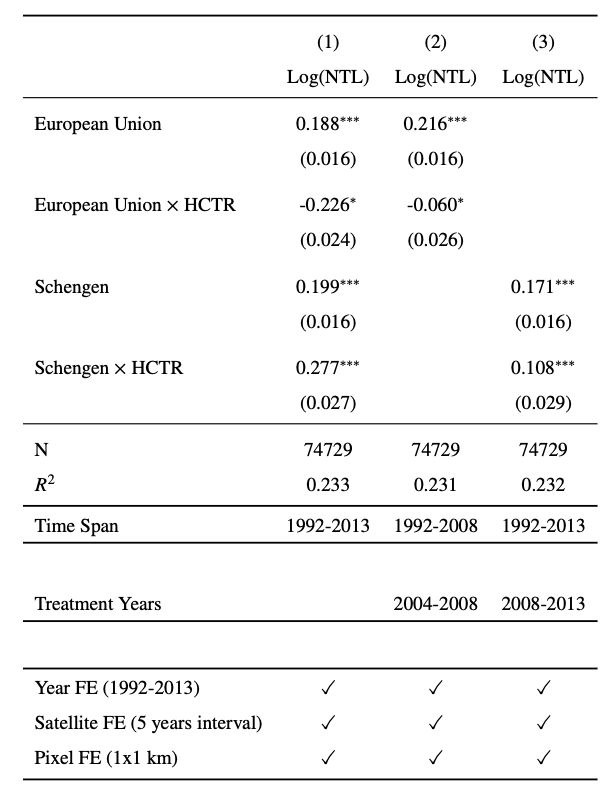
\includegraphics[scale=0.4]{tab2.png}
\end{figure}


\end{frame}

\begin{frame}{\small Result II:
\The Effect of European Division and Integration on Business Establishments}
\justifying
\centering
\scriptsize (1) During the period of division, the market concentration shifted away from the pre-division center. (2) After the EU enlargement, this trend persisted. (3) However, following the Schengen enlargement, pre-division centers began to return to their original state, with a notable increase in the establishment of firms close vicinity.

%A three-way panel dataset that captures the establishment of firms within 500m x 500m blocks over the century from 1900 to 2020. This dataset includes information on the firms, the blocks where they are located, and their corresponding year of establishment.

\begin{figure}
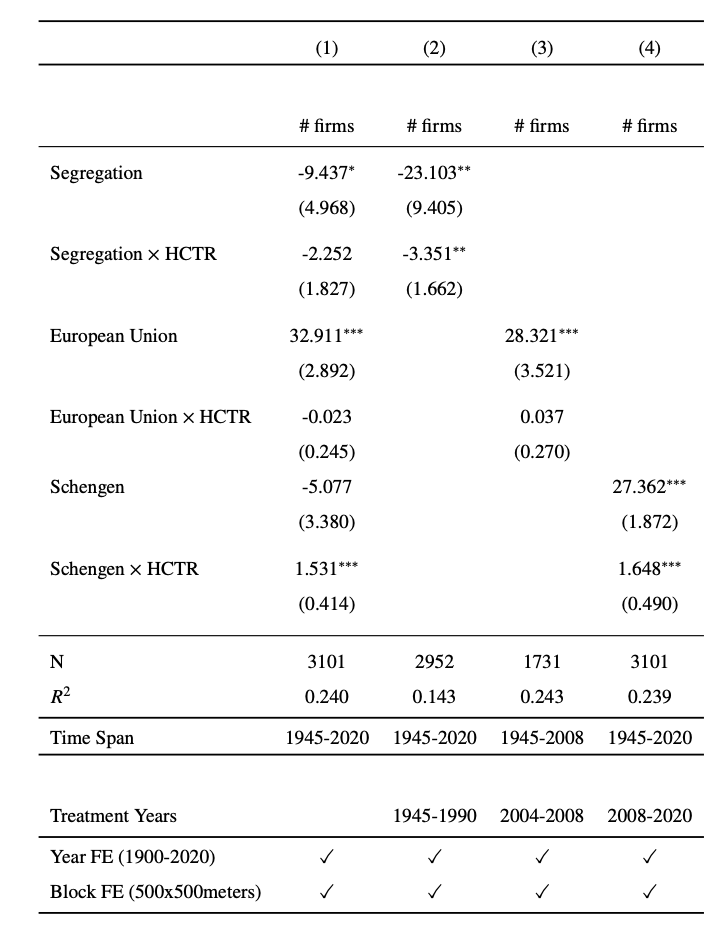
\includegraphics[scale=0.4]{tab3.png}
\end{figure}
\end{frame}


\begin{frame}{Channels}
Identify two key channels that shaped market concentration after the removal of all border barriers between divided European border cities in 2008.
\vspace{0.6cm}
\begin{itemize}
    \item \textbf{Cultural Factors}: language \& cultural similarities
    \item \textbf{Economic Sectors}: consumer \& producer oriented
    \vspace{0.3cm}
\end{itemize}
\end{frame}

\begin{frame}{\small Channel I: 
\\Language and Cultural Similarities}
\justifying
\centering
\small Linguistic proximity between divided cities, whether through a shared or similar language with neighboring areas, promotes stronger economic concentration near the pre-division centers.
\begin{figure}
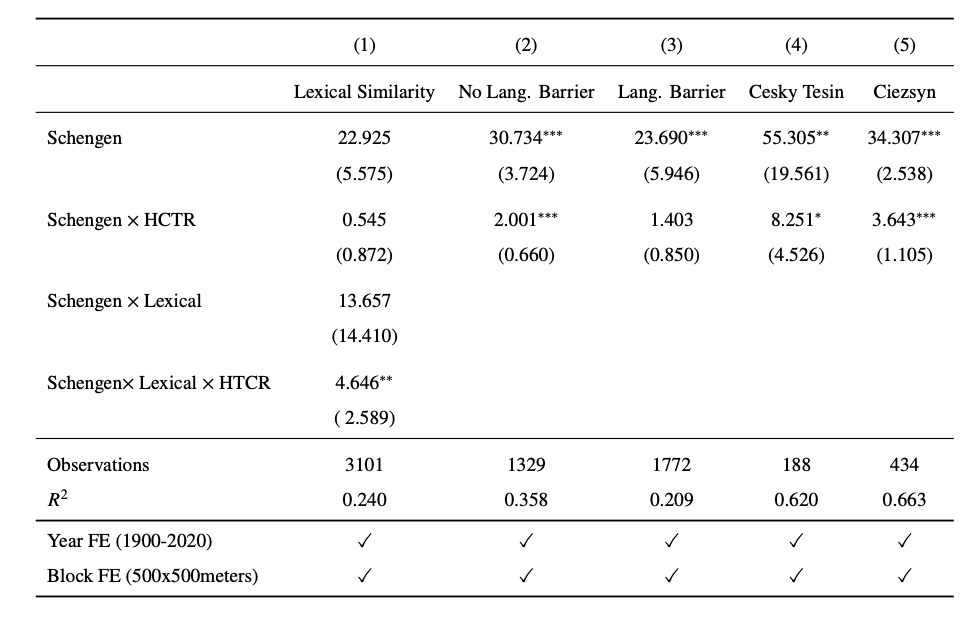
\includegraphics[scale=0.6]{tab4.png}
\end{figure}
\end{frame}

\begin{frame}{\small Channel II: \\Sectoral Distribution of Newly Established Firms in Divided Cities (1900-2022)}
\justifying
Pre-division centers became more attractive for activities centered with cultural, historical, and entertainment aspects, making them particularly attractive to consumer-oriented companies.
\centering
\begin{figure}
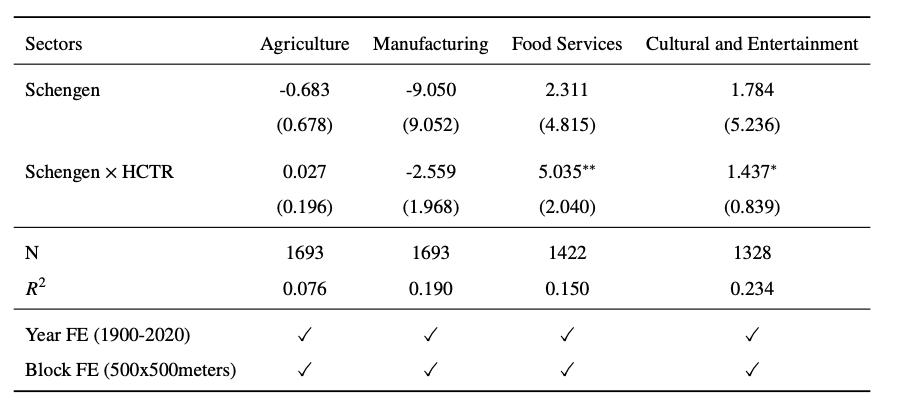
\includegraphics[scale=0.7]{tab5.png}
\end{figure}
\end{frame}


\begin{frame}{Take-aways}
The 2004 EU enlargement proved insufficient to redistribute economic activities effectively. Economic concentration became more pronounced only after the 2008 Schengen enlargement, which allowed for the free movement of people across borders.
\vspace{1cm}
\begin{itemize}
\item Language plays a significant role.  
\item The dynamics of consumers is crucial.  
\item  Historical memory is of even greater importance.  
\end{itemize}  
\end{frame}



\begin{frame}{Thank You}
\vspace{0.5cm}
\textit{email}:  ketevani.kapanadze@eruni.org
\\ 
\textit{web}: www.ketevanikapanadze.com
\end{frame}

\begin{comment}
\begin{frame}[label=frankfurt]{Frankfurt (DE) - Slubice (PL)}
\Acrobatmenu{GoBack}{\leftarrow}
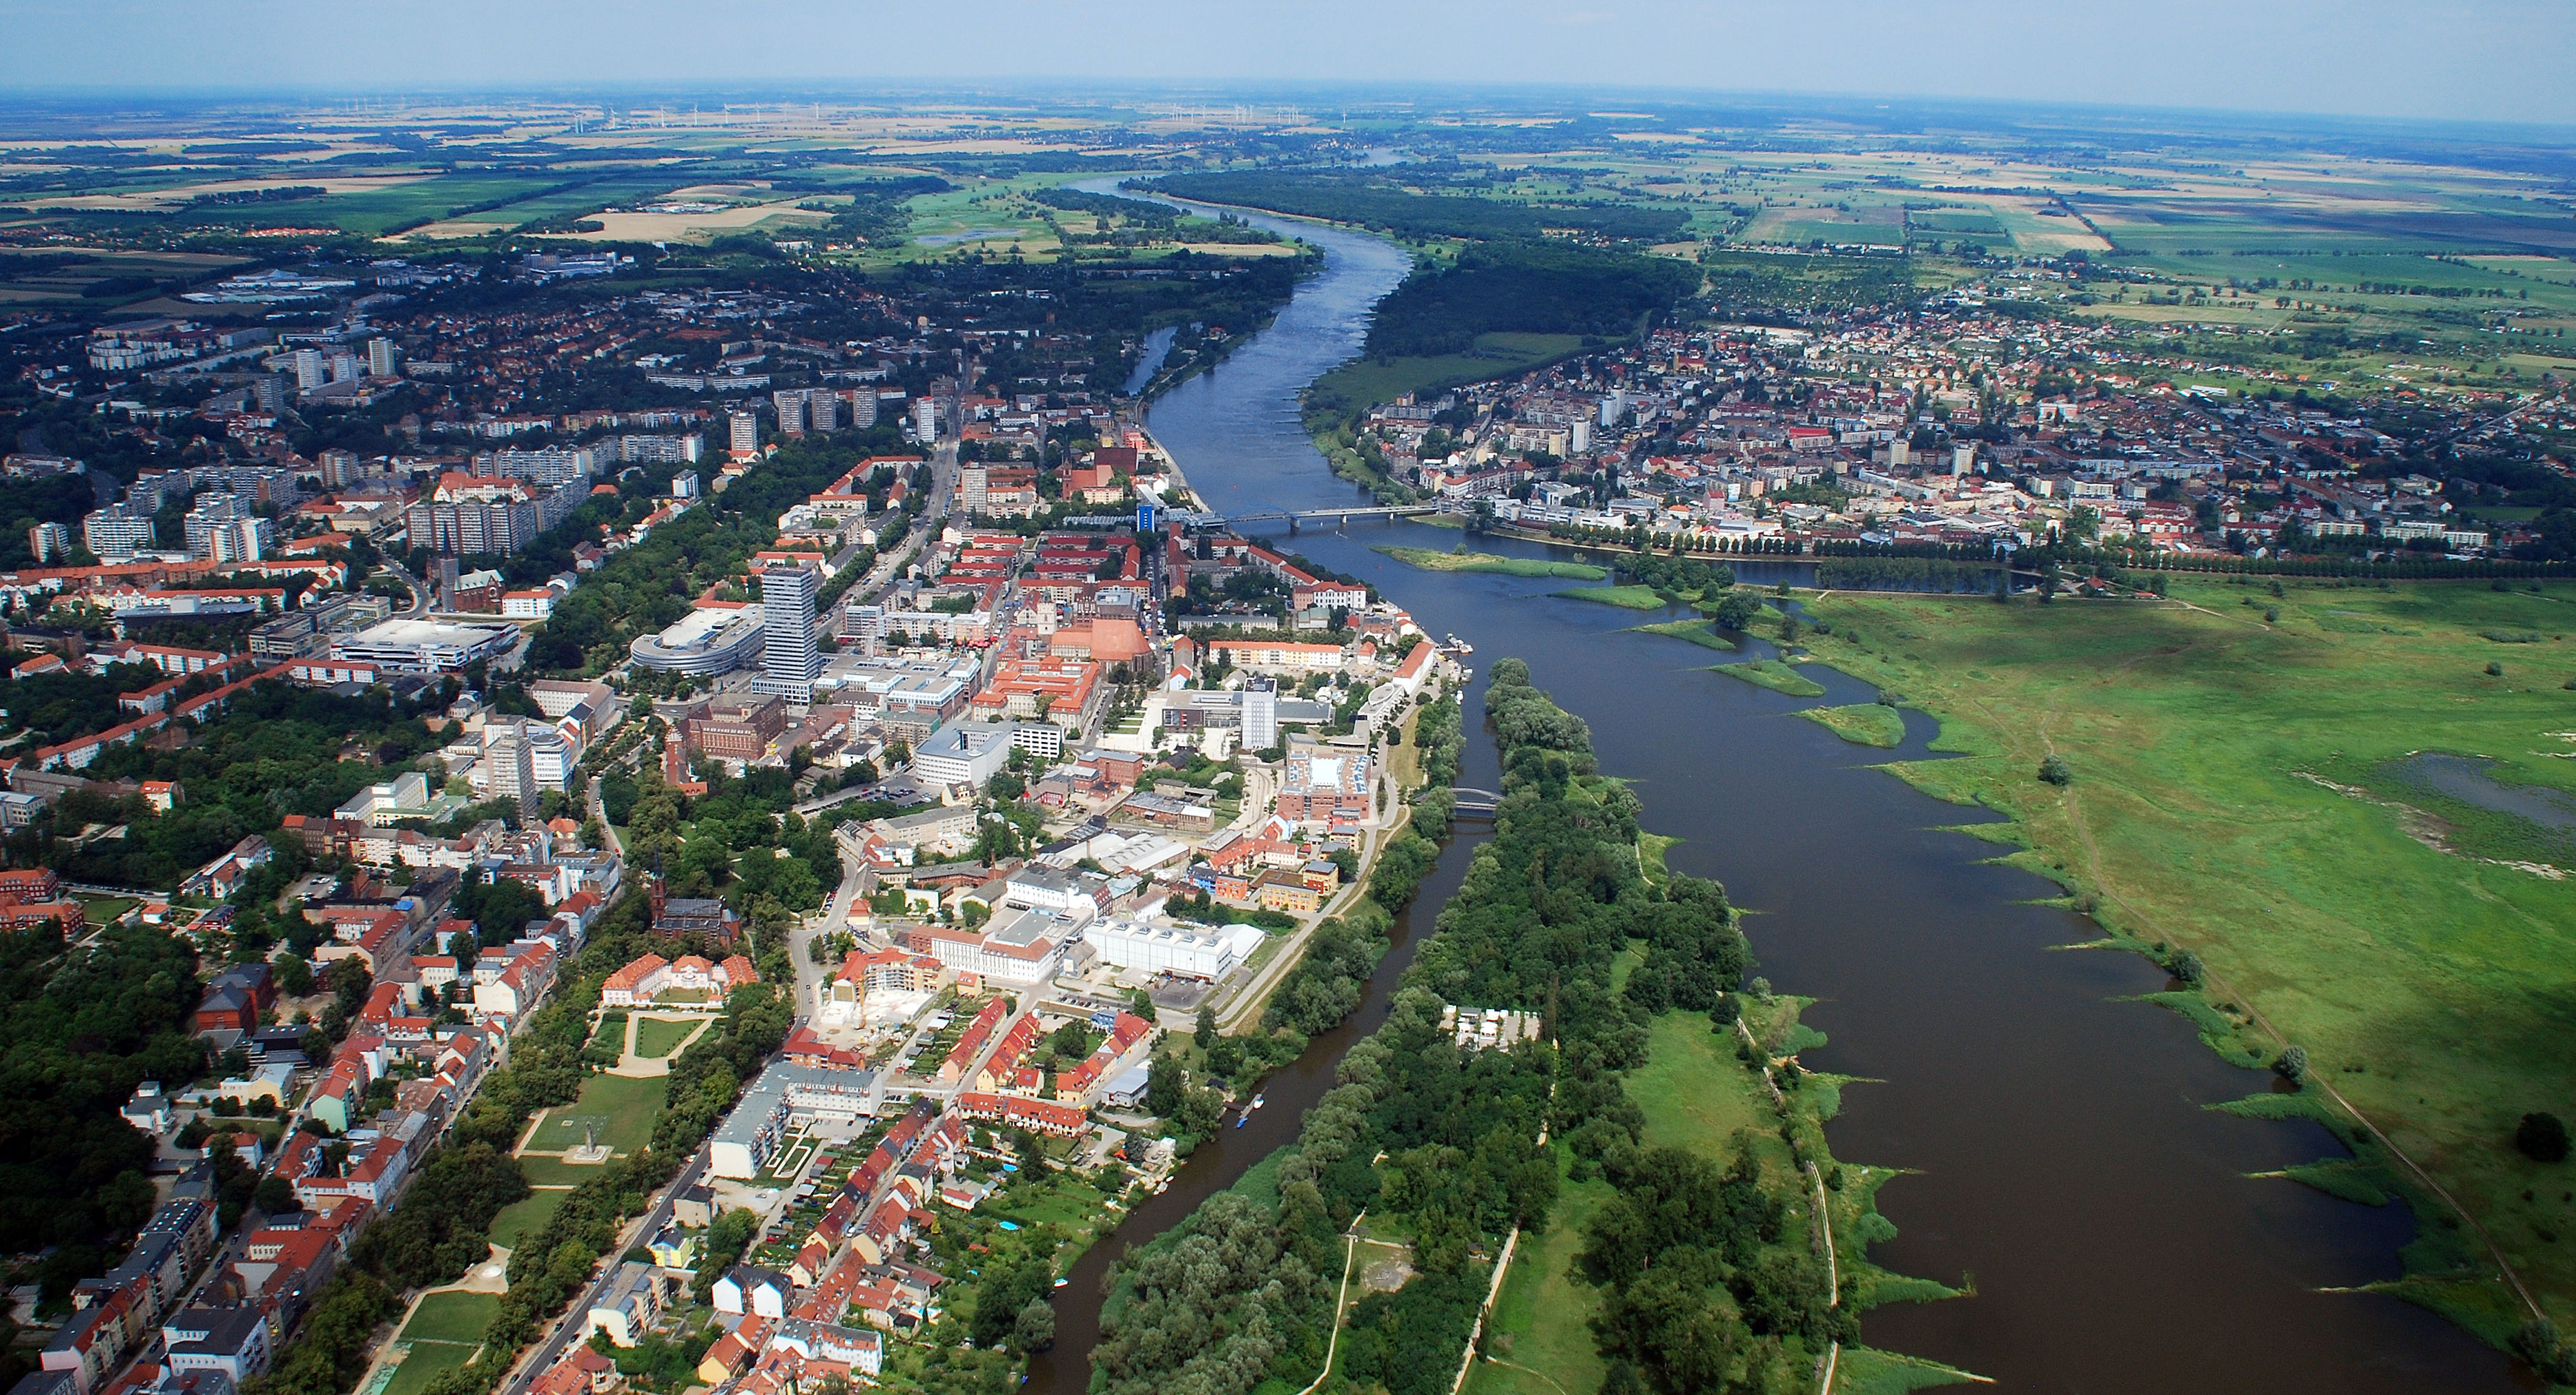
\includegraphics[scale=0.3]{frankfurt slubice.jpg}
\end{frame}


\begin{frame}[label=tesin]{Cesky Tesin (CZ) - Cieszyn (PL)}
\Acrobatmenu{GoBack}{\leftarrow}
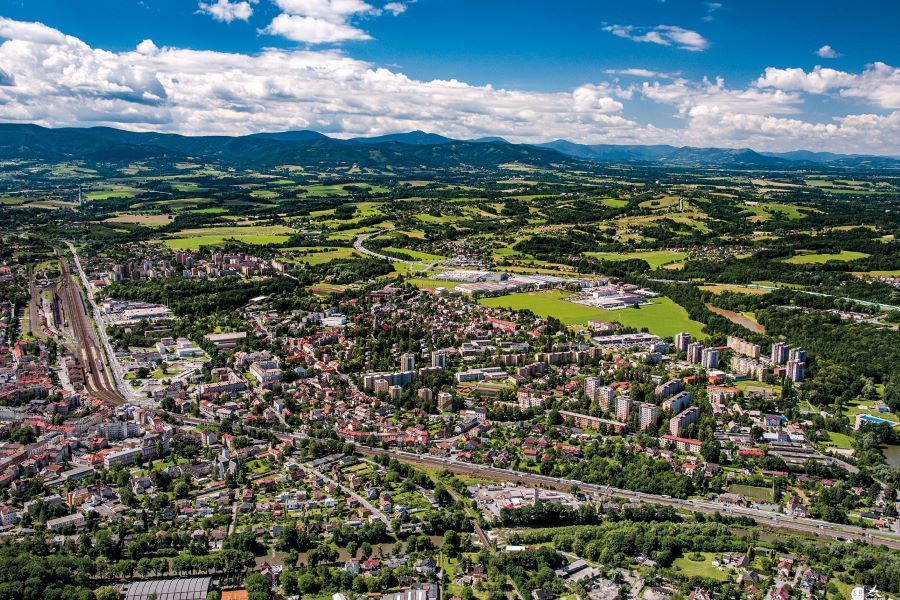
\includegraphics[scale=0.3]{tesin vs ciezsyn.jpg}
\end{frame}
\end{comment}

\end{document}